\documentclass[10pt]{IEEEtran}
\usepackage[T1]{fontenc}
\usepackage{etex}
\usepackage{epsfig}
\usepackage{amsmath}
\usepackage{multirow}
\usepackage{tabularx}
\usepackage{booktabs}
\usepackage{amsmath,graphicx}
\usepackage{pgf}
\usepackage{tikz}
\usepackage{subfig}
\usetikzlibrary{backgrounds,shapes,snakes}
\usetikzlibrary{calc,chains,positioning}
\usepackage{phaistos}
\usepackage{cases}
\usepackage{pgfplots}
%\usepackage{empheq}
\usepackage{cite}
\parindent=0pt

\begin{document}

\newlength\figureheight
\newlength\figurewidth
\setlength\figureheight{2.3cm}
\setlength\figurewidth{0.37\textwidth}

%
\title{Joint Dereverberation and Noise Reduction \\ based on Acoustic Multi-Channel Equalization}

\author{%
  Ina~Kodrasi,~\IEEEmembership{Student~Member,~IEEE} and Simon~Doclo,~\IEEEmembership{Senior Member,~IEEE}
  \thanks{The authors are with the Signal Processing Group, Department of Medical Physics and Acoustics, and Cluster of Excellence Hearing4All, University of Oldenburg, Germany (e-mail: ina.kodrasi@uni-oldenurg.de, simon.doclo@uni-oldenburg.de).}%
  \thanks{This work was supported in part by a Grant from the GIF, the German-Israeli Foundation for Scientific Research and Development, the Cluster of Excellence 1077 Hearing4All funded by the German Research Foundation (DFG), and the Marie Curie Initial Training Network DREAMS (Grant no. 316969).}%
}
% make the title area
\maketitle
\newpage

\begin{abstract}
\boldmath
Regularized acoustic multi-channel equalization techniques, such as regularized partial multi-channel equalization based on the multiple-input/output inverse theorem~(RPMINT), are able to achieve a high dereverberation performance in the presence of room impulse response perturbations but may lead to amplification of the additive noise.
In this paper two time-domain techniques aiming at joint dereverberation and noise reduction based on acoustic multi-channel equalization are proposed.
The first technique, namely RPMINT for joint dereverberation and noise reduction~(RPM-DNR), extends RPMINT by explicitly taking the noise statistics into account.
In addition to the regularization parameter used in RPMINT, the RPM-DNR technique introduces an additional weighting parameter, enabling a trade-off between dereverberation and noise reduction.
The second technique, namely multi-channel Wiener filter for joint dereverberation and noise reduction~(MWF-DNR), takes both the speech and the noise statistics into account and uses the RPMINT filter to compute a dereverberated reference signal for the multi-channel Wiener filter.
The MWF-DNR technique also introduces an additional weighting parameter, which now provides a trade-off between speech distortion and noise reduction.
To automatically select the regularization and weighting parameters, for the RPM-DNR technique a novel procedure based on the L-hypersurface is proposed, whereas for the MWF-DNR technique two decoupled optimization procedures based on the L-curve are used.
Extensive simulations demonstrate using instrumental measures that the RPM-DNR technique maintains the dereverberation performance of the RPMINT technique while improving its noise reduction performance.
Furthermore, it is shown that the MWF-DNR technique yields a significantly better noise reduction performance than the RPM-DNR technique at the expense of a worse dereverberation performance.
\end{abstract}
\begin{IEEEkeywords}
acoustic multi-channel equalization, dereverberation, noise reduction, automatic parameter selection, L-hypersurface
\end{IEEEkeywords}

\section{Introduction}
g\IEEEPARstart{I}{N} many hands-free speech communication applications, such as teleconferencing, voice-controlled systems, or hearing aids, the recorded microphone signals do not only contain the desired speech signal, but also attenuated and delayed copies of the desired speech signal due to reverberation, as well as additive noise.
Reverberation and noise cause the recorded signals to sound distant and spectrally distorted, and typically result in a degradation of speech intelligibility and a performance deterioration of automatic speech recognition systems~\cite{Omologo_1998,Beutelmann_2006}.
With the continuously growing demand for high-quality hands-free communication, speech enhancement techniques aiming at joint dereverberation and noise reduction have become indispensable.
In the last decade, both single- as well as multi-channel techniques have been proposed, with multi-channel techniques being generally preferred since they enable to exploit both the spectro-temporal and the spatial characteristics of the received microphone signals.
Existing dereverberation techniques can be broadly classified into spectral enhancement techniques~\cite{Lebart_ACUSTICA_2001,Habets_ICASSP_2005,Habets2009a,Kuklasinski_EUSIPCO_2014}, probabilistic modeling-based techniques~\cite{Nakatani_ITASLP_2010,Jukic_ICASSP_2014,Schwartz_ITASLP_2015}, and acoustic multi-channel equalization techniques~\cite{Miyoshi_ITASS_1988, Kallinger_ICASSP_2006,Jungmann_ITASLP_2012, Kodrasi_ITASLP_2013, Lim_ITASLP_2014, Rashobh_ITASLP_2014}.

Spectral enhancement techniques aim to suppress the late reverberation in the spectral domain by estimating the late reverberant power spectral density, e.g., based on an exponentially decaying room impulse response~(RIR) model~\cite{Lebart_ACUSTICA_2001,Habets_ICASSP_2005,Habets2009a} or a diffuse sound field model~\cite{Kuklasinski_EUSIPCO_2014}.
Such techniques have been extended to achieve joint dereverberation and noise reduction typically by using a two-stage approach.
A commonly used two-stage approach is based on the decomposition of the multi-channel Wiener filter~(MWF) into a minimum variance distortionless response~(MVDR) beamformer and a single-channel postfilter~\cite{Simmer_book_2001}. 
The MVDR beamformer is applied to reduce the noise and some reverberation, whereas the single-channel postfilter is used to suppress the residual noise and reverberation at the MVDR output~\cite{Braun_EUSIPCO_2013,Cauchi_Reverb_2014}. 
In~\cite{Habets_ITASLP_2013} another two-stage beamforming approach to joint dereverberation and noise reduction was proposed, which does not explicitly model and estimate the late reverberant power spectral density but nevertheless relies on the assumption of a diffuse sound field model for the late reverberation. 
Based on this assumption, in the first stage a superdirective beamformer is applied to generate a dereverberated reference signal, whereas in the second stage the MWF is used to achieve noise reduction.

Probabilistic modeling-based techniques generally model the acoustic transfer function either as an auto-regressive process~\cite{Nakatani_ITASLP_2010,Jukic_ICASSP_2014} or using the convolutive transfer function model~\cite{Schwartz_ITASLP_2015}, whereas the clean speech spectral coefficients are modeled using, e.g., a Gaussian~\cite{Nakatani_ITASLP_2010} or a Laplacian distribution~\cite{Jukic_ICASSP_2014}.
Dereverberation is then performed by maximum likelihood estimation of all unknown model parameters. 
In addition, by modeling the noise spectral coefficients, probabilistic modeling-based techniques have also been proposed for joint dereverberation and noise reduction~\cite{Yoshioka_ITASLP_2009,Ito_ICASSP_2014}.

Acoustic multi-channel equalization techniques aim to reshape the available RIRs~(measured or estimated) between the speech source and the microphone array. 
These techniques in principle comprise an attractive approach to speech dereverberation since in theory perfect dereverberation can be achieved~\cite{Miyoshi_ITASS_1988,Hacihabibouglu_ITASLP_2012}.
A well-known acoustic multi-channel equalization technique which aims at perfect dereverberation is the multiple-input/output inverse theorem~(MINT) technique~\cite{Miyoshi_ITASS_1988}, which however suffers from several drawbacks in practice. 
Since the available RIRs typically differ from the true RIRs due to fluctuations~(e.g., temperature or position variations~\cite{Radlovic_ITSA_2000}), due to the sensitivity of blind system identification~(BSI) methods to near-common zeros or interfering noise~\cite{Haque_SPL_2008,Lin_ITASLP_2012,Lim_IWAENC_2014}, or due to the sensitivity of supervised system identification~(SSI) methods to interfering noise~\cite{Lim_ITASLP_2014}, MINT fails to invert the true RIRs, possibly leading to severe distortions in the output signal~\cite{Kodrasi_ITASLP_2013,Lim_ITASLP_2014}.
In order to increase the robustness against RIR perturbations, partial multi-channel equalization techniques such as channel shortening~(CS)~\cite{Kallinger_ICASSP_2006}, relaxed multi-channel least-squares~(RMCLS)~\cite{Lim_ITASLP_2014}, and partial multi-channel equalization based on MINT~(PMINT)~\cite{Kodrasi_ITASLP_2013} have been proposed. 
Since early reflections tend to improve speech intelligibility~\cite{Arweiler_JASA_2011} and late reverberation is the major cause of speech intelligibility degradation, the objective of these techniques is to relax the constraints on the reshaping filter design by suppressing only the late reverberation.
To additionally increase the robustness against RIR perturbations, regularization has been incorporated into these techniques in~\cite{Kodrasi_ITASLP_2013}, where the regularization parameter enables a trade-off between dereverberation accuracy and robustness against RIR perturbations.
{{In~\cite{Kodrasi_ITASLP_2013} it has been experimentally validated that the regularized PMINT~(RPMINT) technique outperforms the regularized CS and regularized RMCLS techniques in terms of dereverberation performance.}}
However, even though partial acoustic multi-channel equalization techniques are able to achieve a high dereverberation performance in a noiseless scenario, in the presence of additive noise this noise may even be amplified, since the noise statistics are not explicitly taken into account in the reshaping filter design~\cite{Kodrasi_ITASLP_2013,Thomas_WASPAA_2011}. 

In this paper, we propose two time-domain techniques to achieve joint dereverberation and noise reduction based on acoustic multi-channel equalization. 
{{The first technique, namely RPMINT for joint dereverberation and noise reduction~(RPM-DNR), extends RPMINT by explicitly taking the noise statistics into account.}}
In addition to the regularization parameter used in RPMINT, the RPM-DNR technique introduces an additional weighting parameter, enabling a trade-off between dereverberation and noise reduction performance. 
The second technique, namely MWF for joint dereverberation and noise reduction~(MWF-DNR), takes both the speech and the noise statistics into account and uses the RPMINT filter to compute a dereverberated reference signal for the MWF.
{{The reason behind using the RPMINT filter to compute a dereverberated reference signal for the MWF-DNR technique lies in the high dereverberation performance of the RPMINT technique, as has been experimentally validated in~\cite{Kodrasi_ITASLP_2013}.}}
Similarly to the RPM-DNR technique, the MWF-DNR technique also introduces a weighting parameter, now enabling a trade-off between speech distortion and noise reduction, with speech distortion being the deviation of the output speech signal from the dereverberated reference signal.
Some preliminary results for the MWF-DNR technique have been presented in~\cite{Kodrasi_IWAENC_2014}.
{{The optimal regularization and weighting parameters yielding the best performance for the proposed RPM-DNR and MWF-DNR techniques can only be determined intrusively, i.e., exploiting knowledge of the true RIRs and the true speech and noise statistics, limiting their practical applicability.
In this paper we therefore also propose a novel automatic procedure based on the L-hypersurface~\cite{Belge_SPIE_1998} for jointly selecting the regularization and weighting parameters in the RPM-DNR technique.}}
To automatically select the regularization and weighting parameters in the MWF-DNR technique it is proposed to use two decoupled optimization procedures based on the L-curve~\cite{Hansen_1993}.
Extensive simulations for different levels of additive noise, RIR perturbations, and correlation matrix estimation errors show by means of instrumental measures that the RPM-DNR technique can achieve a better noise reduction performance while not degrading the dereverberation performance of the RPMINT technique.
Furthermore, it is shown that the MWF-DNR technique yields a significantly better noise reduction performance than the RPM-DNR technique at the expense of a worse dereverberation performance~(depending on the correlation matrix estimation errors).

The paper is organized as follows. 
In Section~\ref{sec: conf} the considered acoustic configuration and the used notation is introduced.
In Section~\ref{sec: eq} state-of-the-art acoustic multi-channel equalization techniques are briefly reviewed. 
In Section~\ref{sec: nr} two novel time-domain techniques for joint dereverberation and noise reduction based on acoustic multi-channel equalization are proposed, for which automatic procedures for selecting the regularization and weighting parameters are proposed in Section~\ref{sec: auto}.
The dereverberation and noise reduction performance of all considered techniques is extensively compared in Section~\ref{sec: exp} using instrumental measures.

\section{Configuration and Notation}
\label{sec: conf}
We consider a reverberant and noisy acoustic system with a single speech source and $M$ microphones, as depicted in Fig.~\ref{fig: conf}.
\begin{figure}[b!]
  \centering
  %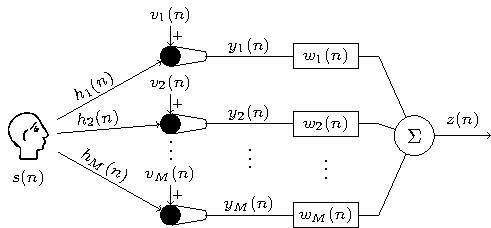
\includegraphics[width = 0.4\textwidth,height = 3cm]{Plots2/configuration.pdf}
  \tikzset{>=latex}

  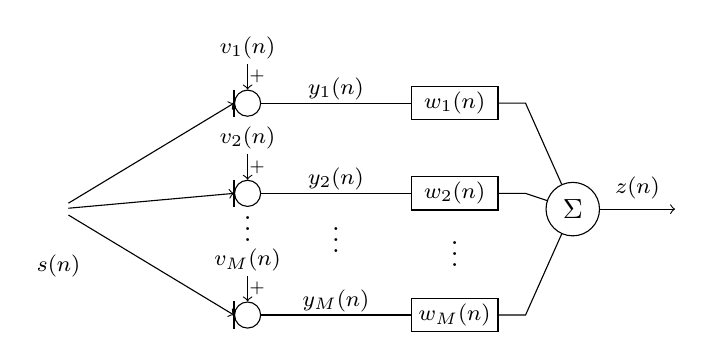
\begin{tikzpicture}
    % Adjustments
    \def\micd{.1cm}                % mic diameter
    \def\micl{.6cm}                % mic length
    \def\micw{.15cm}                % mic width
    \def\micbend{10}               % mic bottom bend
    \def\micdistance{.8cm}         % distance between microphones
    \def\filterdistance{1.9cm}     % distance between microphone and filter
    \def\filteroutline{.9cm}       % length of line which gets out of filter
    \def\sumdistance{1.5cm}        % distance of sum node to the filter
    \def\sumoutline{1cm}           % length of line which gets out of sum
    \def\headdistance{2.4cm}       % distance between microphone and head
%
    % Styles
    \tikzset{%
      mic head/.style={fill=white,draw=black,circle,minimum size=\micd},
      filter/.style={draw,minimum width=1.1cm,inner sep=2pt},
      sum/.style={draw,circle},
      xlabel/.style={inner sep=1pt,above,midway},
      sumlabel/.style={xlabel},
      hlabel/.style={xlabel,sloped,pos=.4},
      head/.style={font=\Large}
    }   %
    % Draw Microphones
    \begin{scope}[start chain=going below,every node/.style={on chain},node distance=\micdistance]
      \node[mic head] (mic1) {};
      \node[mic head] (mic2) {};
      \node[mic head,yshift=-0.5*\micdistance] (mic3) {};
    \end{scope}
    \node[yshift=12pt] at ($(mic2)!.5!(mic3)$) {$\vdots$};
    %
    \foreach \m in {1,2,3} {%
      \draw (mic\m.north -| mic\m.west) -- (mic\m.south -| mic\m.west);
     %\coordinate (m1) at ($(mic\m)+(\micl,\micw/2)$);
     %\coordinate (m2) at ($(mic\m)+(\micl,-\micw/2)$);
     %\draw (tangent cs:node=mic\m,point={(m1)},solution=1) -- (m1) to[bend left=\micbend] (m2) -- (tangent cs:node=mic\m,point={(m2)},solution=2);
    }%
    % Draw Filter
    \foreach \m/\i in {1/1,2/2,3/M} {%
      \node[filter,right=\filterdistance of mic\m] (filter\m) {\footnotesize $w_{\i}(n)$};
      \draw (mic\m.east) to node[xlabel] (x\m) {\footnotesize $y_{\i}(n)$} (filter\m);
    }
    \node[yshift=3pt] at ($(filter2)!.5!(filter3)$) {$\vdots$};
    \node[yshift=3pt] at ($(x2)!.5!(x3)$) {$\vdots$};
    % Sum Node
    \node[sum] (sum) at ($(filter1)!.5!(filter3)+(\sumdistance,0)$) {$\Sigma$};
    \draw[->] (sum) -- node[above] {\footnotesize $z(n)$} ++(1.3,0);
    % Connect filter with sum
    \foreach \m in {1,2,3} {%
      \draw (filter\m) -- ++(\filteroutline,0) -- (sum);
    }%
    % Head
    \node[head] (head) at ($(mic1)!.5!(mic3)-(\headdistance,0)$) {\PHtattooedHead};
    \node[fill=white,minimum width=4.8pt,minimum height=5.7pt,inner sep=0pt] at ($(head.center)+(2.3pt,-2.5pt)$) {};
    \node at ($(head.center)+(0.0pt,-20.5pt)$) {\footnotesize $s(n)$};
    % Connect head with mics
    \foreach \m/\i in {1/1,2/2,3/M} {%
%      \draw[->] (head) -- node[hlabel] {\footnotesize $h_{\i}(n)$} (mic\m);
      \draw[->] (head) --  (mic\m.west);
    }
    % Draw noise
    \draw[<-] (mic1) -- node[above=0.1cm] {\footnotesize $v_1(n)$} node[right = -0.1cm] {\footnotesize ${}_{+}$} ++(0,0.5);
    \draw[<-] (mic2) -- node[above=0.1cm] {\footnotesize $v_2(n)$} node[right = -0.1cm] {\footnotesize ${}_{+}$} ++(0,0.5);
    \draw[<-] (mic3) -- node[above=0.1cm] {\footnotesize $v_M(n)$} node[right = -0.1cm] {\footnotesize ${}_{+}$} ++(0,0.5);
  \end{tikzpicture}
  \caption{Acoustic system configuration.}
  \label{fig: conf}
\end{figure}
The $m$-th microphone signal $y_m(n)$, $m = 1, \ldots, M,$ at time index $n$ is given by
\begin{align}
\label{eq: y(n)}
y_m(n) & = \sum_{l=0}^{L_h-1} h_m(l)  s(n-l) + v_m(n) \\
& = x_m(n) + v_m(n), 
\end{align}
where $h_m(l), \; l = 0, \; \ldots, \; L_h-1$, are the coefficients of the $L_h$-taps long RIR between the speech source and the $m$-th microphone, $s(n)$ is the clean speech signal, $x_{m}(n)$ is the reverberant speech component, and $v_{m}(n)$ is the additive noise component. 
Denoting the direct path and early reflections of the RIR by $h_{{\rm{d}},m}(l)$ and the late reverberant tail by $h_{{\rm{r}},m}(l)$, the $m$-th microphone signal in~(\ref{eq: y(n)}) can also be expressed as
\begin{align}
y_m(n) & \!\!= \!\!\!\sum_{l=0}^{L_{\rm{d}}-1}h_{{\rm{d}},m}(l) s(n\!-\!l) + \!\!\!\!\!\sum_{l=0}^{L_h\!-\!L_{\rm{d}}\!-\!1}\!\!\!h_{{\rm{r}},m}(l) s(n\!-\!l) + v_m(n) \nonumber \\ 
\label{eq: ysp}
& \!\! = x_{{\rm{d}},m}(n) + x_{{\rm{r}},m}(n) + v_m(n),
\end{align}
where $L_{\rm{d}}$ denotes the length of the direct path and early reflections, $x_{{\rm{d}},m}(n)$ is the $m$-th direct speech component, and $x_{{\rm{r}},m}(n)$ is the $m$-th late reverberant speech component.
Using the filter-and-sum structure in Fig.~\ref{fig: conf}, the output signal $z(n)$ is equal to the sum of the filtered microphone signals, i.e.,
\begin{align}
  z(n) & =\!\! \sum_{m=1}^{M}\!\! \sum_{l=0}^{L_w-1}  w_m(l)x_m(n-l) + \sum_{m=1}^{M} \!\! \sum_{l=0}^{L_w-1}w_m(l)v_m(n-l) \nonumber \\
  \label{eq: outcomp}
  & = z_x(n) + z_v(n),
\end{align}
where $w_m(l), \; l = 0, \; \ldots, \; L_w-1$, are the coefficients of the $L_w$-taps long filter applied to the $m$-th microphone, $z_x(n)$ is the output speech component, and $z_v(n)$ is the output noise component.
The output speech component can also be written as
\begin{align}
z_x(n) & = \!\!\sum_{m=1}^{M}\!\! \sum_{l=0}^{L_w-1} \!\!\!w_m(l)x_{{\rm{d}},m}(n\!-\!l)\! + \!\sum_{m=1}^{M}\!\! \sum_{l=0}^{L_w-1}\!\!\! w_m(n)x_{{\rm{r}},m}(n\!-\!l) \nonumber  \\
\label{eq: zxdzxr}
& = z_{\rm{d}}(n) + z_{\rm{r}}(n),
\end{align}
with $z_{\rm{d}}(n)$ the output direct speech component and $z_{\rm{r}}(n)$ the output late reverberant speech component.
% In the remainder of this paper, the sum of the filtered RIRs will be referred to as the equalized impulse response~(EIR) $c(n)$, i.e.,
% \begin{equation}
% \label{eq: eir}
% c(n) = \sum_{m=1}^M h_m(n) \ast w_m(n).
% \end{equation}

In vector notation, the RIR $\mathbf{h}_m$ and the filter $\mathbf{w}_m$ can be described as 
\begin{align}
\mathbf{h}_m  & = [h_m(0) \; h_m(1) \; \ldots \; h_m(L_h-1)]^T, \\
\mathbf{w}_m  & = [w_m(0) \; w_m(1) \; \ldots \; w_m(L_w-1)]^T.
\end{align}
%where $L_h$ and $L_w$ denote the RIR and the filter length respectively.
Using the $M L_w$-dimensional stacked filter vector $\mathbf{w} = [\mathbf{w}^T_1 \; \mathbf{w}^T_2 \; \ldots \; \mathbf{w}^T_M]^T$, the equalized impulse response~(EIR) vector $\mathbf{c}$ of length $L_c = L_h + L_w - 1$, i.e., $\mathbf{c} = [c(0) \; c(1) \; \ldots \; c(L_c-1)]^T$, can be expressed as
\begin{equation}
\label{eq: eir}
\mathbf{c} = \mathbf{H}\mathbf{w},
\end{equation}
with $\mathbf{H}$ being the $L_c \times ML_w$-dimensional multi-channel convolution matrix, i.e., $\mathbf{H}  = [\mathbf{H}_1 \; \mathbf{H}_2 \; \ldots \; \mathbf{H}_M]$, and
\begin{equation}
\mathbf{H}_m \! = \! \begin{bmatrix}
    h_m(0) & 0 &  \ldots & 0 \\
    h_m(1) & h_m(0) & \ddots & \vdots \\
    \vdots & h_m(1) & \ddots & 0 \\
    h_m(L_h\!-\!1) & \vdots & \ddots & h_m(0) \\
    0 & h_m(L_h\!-\!1) & \ddots & h_m(1) \\
    \vdots & \ddots & \ddots & \vdots \\
    0 & \ldots & 0 & h_m(L_h\!-\!1)
   \end{bmatrix}.
 \end{equation}
Using the $ML_w$-dimensional stacked vector of the microphone signals $\mathbf{y}(n)$, i.e.,
\begin{equation}
\mathbf{y}(n) = \mathbf{x}(n) + \mathbf{v}(n), 
\end{equation}
with
\begin{align}
  \label{eq: y}
  \mathbf{y}(n) &= [\mathbf{y}^T_1(n) \; \mathbf{y}^T_2(n) \; \ldots \; \mathbf{y}^T_M(n)]^T, \\
  \label{eq: y_m}
  \mathbf{y}_m(n) &= [y_m(n) \; y_m(n-1) \; \ldots \; y_m(n-L_w+1)]^T,
\end{align}
and $\mathbf{x}(n)$ and $\mathbf{v}(n)$ similarly defined as in~(\ref{eq: y}) and~(\ref{eq: y_m}), the output signal can be expressed in vector notation as
\begin{equation}
z(n) =  \mathbf{w}^T \mathbf{x}(n) + \mathbf{w}^T \mathbf{v}(n) =  (\underbrace{\mathbf{H}\mathbf{w}}_{\mathbf{c}})^T \mathbf{s}(n) + \mathbf{w}^T \mathbf{v}(n),
\end{equation}
with $\mathbf{s}(n) = [s(n) \; s(n-1) \; \ldots \; s(n-L_c+1)]^T$ and 
\begin{equation}
\label{eq: x}
\mathbf{x}(n) = \mathbf{H}^T\mathbf{s}(n).
\end{equation}
The correlation matrices of $\mathbf{x}(n)$, $\mathbf{v}(n)$, and $\mathbf{y}(n)$ are defined as
\begin{align}
\mathbf{R}_{\mathbf{x}}  &= {\cal{E}} \{\mathbf{x}(n)\mathbf{x}^T(n) \},\\
\mathbf{R}_{\mathbf{v}} & = {\cal{E}} \{\mathbf{v}(n)\mathbf{v}^T(n) \}, \\
\mathbf{R}_{\mathbf{y}} &= {\cal{E}} \{\mathbf{y}(n)\mathbf{y}^T(n)\},
\end{align}
with ${\cal{E}}$ denoting the expected value operator.
Using~(\ref{eq: x}), the reverberant speech correlation matrix $\mathbf{R}_{\mathbf{x}}$ can be expressed as
\begin{equation}
\label{eq: rxs}
\mathbf{R}_{\mathbf{x}} = {\cal{E}} \{\mathbf{H}^T\mathbf{s}(n)\mathbf{s}^T(n)\mathbf{H} \} =  \mathbf{H}^T\mathbf{R}_{\mathbf{s}}\mathbf{H},
\end{equation}
with $\mathbf{R}_{\mathbf{s}}$ being the clean speech correlation matrix.
Assuming that the speech and the noise components are uncorrelated, $\mathbf{R}_{\mathbf{y}} = \mathbf{R}_{\mathbf{x}} + \mathbf{R}_{\mathbf{v}}$.
For conciseness, the time index $n$ will be omitted when possible in the remainder of this paper.

\section{Acoustic Multi-channel Equalization}
\label{sec: eq}
Acoustic multi-channel equalization techniques aim only at speech dereverberation by designing a reshaping filter $\mathbf{w}$ such that the resulting EIR in~(\ref{eq: eir}) equals a target dereverberated EIR $\mathbf{c}_t$, where typically the presence of the additive noise $\mathbf{v}(n)$ is completely disregarded.
{{In practice, only perturbed RIRs $\hat{h}_m$ are available, i.e., $\hat{h}_m = h_m + e_m$, where $e_m$ represents the RIR perturbations due to fluctuations~(e.g., temperature or position fluctuations~\cite{Radlovic_ITSA_2000}) or due to the sensitivity of BSI and SSI methods to near-common zeros or interfering noise~\cite{Haque_SPL_2008,Lin_ITASLP_2012,Lim_IWAENC_2014,Lim_ITASLP_2014}.
Hence, for the reshaping filter design the perturbed convolution matrix $\hat{\mathbf{H}} = \mathbf{H} + \mathbf{E}$ is used, where $\mathbf{E}$ represents the convolution matrix of the RIR perturbations.
It should be noted that BSI methods result in a convolutive RIR perturbation instead of an additive one~\cite{Thomas_ICASSP_2012}. 
However, the discussion in the remainder of this paper is independent of the type of perturbations, as long as a model can be developed to characterize these perturbations.}}

In this paper we will focus on the PMINT technique proposed in~\cite{Kodrasi_ITASLP_2013}, which aims at suppressing the late reverberation and preserving the perceptual speech quality.
{{To this purpose, the late reverberant taps of the target EIR $\mathbf{c}_t$ are set equal to $0$, while the remaining taps are set equal to the direct path and early reflections of one of the available RIRs.
Without loss of generality, the RIR of the first microphone, i.e.,  $\hat{\mathbf{h}}_1$, is used to define the target EIR as
\begin{equation}
\label{eq: ct}
\mathbf{c}_t = [\underbrace{0 \; \ldots \; 0}_{\tau} \; \hat{h}_1(0) \; \ldots \; \hat{h}_1(L_{\rm{d}}-1) \; 0 \; \ldots \; 0 ]^{T},
\end{equation}
with $\tau$ a delay introduced to relax the causality constraints on the filter design~\cite{Hikichi_EURASIP_2007}.}}
The PMINT filter is computed by minimizing the least-squares cost function
\begin{equation}
\label{eq: lscost}
J_{_{\rm P}} = \|\hat{\mathbf{H}}\mathbf{w} - \mathbf{c}_t \|_2^2.
\end{equation}
As shown in~\cite{Miyoshi_ITASS_1988}, assuming that the available RIRs do not share any common zeros and using $L_w \geq \lceil{\frac{L_h-1}{M-1}\rceil}$, the PMINT filter minimizing the least-squares error in~(\ref{eq: lscost}) to 0 is equal to
\begin{equation}
\label{eq: lssol}
\mathbf{w}_{_{\rm P}} = \hat{\mathbf{H}}^+\mathbf{c}_t,
\end{equation}
where $\{\cdot \}^+$ denotes the matrix pseudoinverse.
Since the perturbed convolution matrix $\hat{\mathbf{H}}$ is assumed to be a full row-rank matrix, its pseudoinverse can be computed as $\hat{\mathbf{H}}^+ = \hat{\mathbf{H}}^T(\hat{\mathbf{H}}\hat{\mathbf{H}}^T)^{-1}$.
% If $\hat{\mathbf{H}}$ is a square matrix with $L_c = M L_w$, then $\hat{\mathbf{H}}^+ = \hat{\mathbf{H}}^{-1}$ and only one solution to~(\ref{eq: hc}) exists, i.e., $\mathbf{w}_{_{\rm P}} = \hat{\mathbf{H}}^{-1}\mathbf{c}_t$.
% If $\hat{\mathbf{H}}$ is a fat matrix with $L_c < M L_w$, multiple solutions to~(\ref{eq: hc}) exist, with~(\ref{eq: lssol}) yielding the minimum-norm solution~\cite{Golub_Matrix_book}.

When the true RIRs are available, i.e., $\hat{\mathbf{H}} = \mathbf{H}$, the PMINT filter yields perfect dereverberation, i.e., $\mathbf{H} \mathbf{w}_{_{\rm P}} = \mathbf{c}_t$~\cite{Kodrasi_ITASLP_2013}.
However, in the presence of RIR perturbations, applying the PMINT filter to the true convolution matrix yields
\begin{equation}
\label{eq: lsout}
\mathbf{H}\mathbf{w}_{_{\rm P}} = \hat{\mathbf{H}} \mathbf{w}_{_{\rm P}} - \mathbf{E}\mathbf{w}_{_{\rm P}} = \mathbf{c}_t - \mathbf{E}\mathbf{w}_{_{\rm P}}.
\end{equation}
The first term in~(\ref{eq: lsout}) is the target EIR, whereas the second term represents distortions due to RIR perturbations.
In order to increase the robustness of acoustic multi-channel equalization techniques against RIR perturbations, regularized techniques such as the RPMINT technique have been proposed~\cite{Kodrasi_ITASLP_2013}.
As shown in~\cite{Hikichi_EURASIP_2007}, when taking the RIR perturbations into account, an optimal reshaping filter in the minimum mean-square error sense can be computed by minimizing the cost function
\begin{equation}
\label{eq: c_E}
J = \| \hat{\mathbf{H}}\mathbf{w} - \mathbf{c}_t\|_2^2 + \mathbf{w}^T {\cal{E}}\{\mathbf{E}^T\mathbf{E} \}\mathbf{w},
\end{equation}
where it is assumed that ${\cal{E}}\{\mathbf{E} \} = \mathbf{0}$.
The matrix ${\cal{E}}\{\mathbf{E}^T\mathbf{E} \}$ in~(\ref{eq: c_E}) obviously depends on the energy and the type of RIR perturbations, e.g., perturbations arising due to microphone position fluctuations~\cite{Radlovic_ITSA_2000,Jungmann_ITASLP_2012}, or perturbations arising from BSI or SSI methods~\cite{Haque_SPL_2008,Lin_ITASLP_2012,Lim_IWAENC_2014}.
While statistical models can be developed for the correlation structure of different types of perturbations, the exact ${\cal{E}}\{\mathbf{E}^T \mathbf{E} \}$ cannot be known in practice. 
To account for inaccuracies in modeling ${\cal{E}}\{\mathbf{E}^T\mathbf{E} \}$, regularized acoustic multi-channel equalization techniques introduce a regularization parameter $\delta$ and use ${\cal{E}}\{ \mathbf{E}^T \mathbf{E} \} = \delta \mathbf{R}_{e}$, with $\mathbf{R}_{e}$ constructed based on a perturbation model~\cite{Jungmann_ITASLP_2012, Lim_IWAENC_2014}. 
{{When no knowledge about the perturbations is available, they are often assumed to be spatially and temporally white, i.e., ${\cal{E}}\{\mathbf{E}^T \mathbf{E} \} = \delta \mathbf{I}$, with $\mathbf{I}$ denoting the $ML_w \times ML_w$-dimensional identity matrix~\cite{Hikichi_EURASIP_2007,Kodrasi_ITASLP_2013}.
This assumption has been used for the experimental results in Section~\ref{sec: exp}.}}

Using ${\cal{E}}\{ \mathbf{E}^T \mathbf{E} \} = \delta \mathbf{R}_{e}$ in~(\ref{eq: c_E}), the RPMINT cost function is given by~\cite{Kodrasi_ITASLP_2013}
\begin{align}
  \label{eq: rlscost}
  J_{_{\rm RP}} &=  \| \hat{\mathbf{H}}\mathbf{w} - \mathbf{c}_t \|_2^2 + \delta  \mathbf{w}^T \mathbf{R}_{e} \mathbf{w} \\
 &= \epsilon_{{c}} + \delta \epsilon_e,
\end{align}
where $\epsilon_{{c}}$ denotes the dereverberation error energy and $\epsilon_{e}$ denotes the distortion energy due to RIR perturbations.
Clearly, the dereverberation performance, i.e., the deviation of the resulting EIR from the target EIR $\mathbf{c}_t$, depends on both the dereverberation error and distortion energies~(cf.~(\ref{eq: lsout})), and the regularization parameter $\delta$ provides a trade-off between the two.
Minimizing~(\ref{eq: rlscost}) yields the RPMINT filter
\begin{equation}
\label{eq: wrp}
\mathbf{w}_{_{\rm RP}} = (\hat{\mathbf{H}}^T\hat{\mathbf{H}} + \delta \mathbf{R}_{e})^{-1}\hat{\mathbf{H}}^T\mathbf{c}_t,
\end{equation}
where $\delta$ can be automatically computed using the procedure based on the L-curve proposed in~\cite{Kodrasi_ITASLP_2013}~(cf. Section~\ref{sec: auto}).
% As the regularization parameter $\delta$ approaches $0$, it can be shown that
% \begin{equation}
% \label{eq: hreg_h}
% \lim_{\delta \rightarrow 0} \left[ (\hat{\mathbf{H}}^T\hat{\mathbf{H}} + \delta \mathbf{R}_{\mathbf{e}})^{-1}\hat{\mathbf{H}}^T \mathbf{c}_t \right] = \hat{\mathbf{H}}^+\mathbf{c}_t,
% \end{equation}
% and hence, the RPMINT filter in~(\ref{eq: wrp}) is equal to the minimum $l_2$-norm PMINT filter in~(\ref{eq: lssol}), i.e., 
% \begin{equation}
% \lim_{\delta \rightarrow 0} \mathbf{w}_{_{\rm RP}} = \mathbf{w}_{_{\rm P}}.
% \end{equation}
{{While the PMINT filter fails to achieve dereverberation in the presence of RIR perturbations, it has been shown in~\cite{Kodrasi_ITASLP_2013} that the RPMINT filter yields a significantly better dereverberation performance, i.e., 
\begin{equation}
\label{eq: rpperfect}
\mathbf{w}_{_{\rm RP}}^T\mathbf{x} \approx  \mathbf{c}_t^T \mathbf{s},
\end{equation}
outperforming other regularized techniques such as regularized CS and regularized RMCLS.}}
Furthermore, the RPMINT technique is able to partly avoid the noise amplification at the output of the system~\cite{Kodrasi_ITASLP_2013}~(cf. Section~\ref{sec: exp}), however, its noise reduction performance is limited since the actual noise statistics are not explicitly taken into account. 

\section{Joint Dereverberation and Noise Reduction based on  Acoustic Multi-Channel Equalization}
\label{sec: nr}
Since acoustic multi-channel equalization techniques design reshaping filters for dereverberation without taking the presence of additive noise into account, the output noise power $\epsilon_{v}$, i.e., 
\begin{equation}
\label{eq: np}
\epsilon_v = {\cal{E}} \{(\mathbf{w}^T \mathbf{v})^2 \} = \mathbf{w}^T \mathbf{R}_{\mathbf{v}}\mathbf{w},
\end{equation}
is not explicitly controlled and may even be amplified compared to the noise power in the microphone signals.
In this section, two time-domain techniques aiming at joint dereverberation and noise reduction based on acoustic multi-channel equalization are proposed, namely RPMINT for joint dereverberation and noise reduction taking the noise statistics into account~(cf. Section~\ref{sec: rpdnr}) and MWF for joint dereverberation and noise reduction taking both the speech and the noise statistics into account~(cf. Section~\ref{sec: mwfdnr}).

% \subsection{Minimum Variance Distortionless Response Beamformer for Dereverberation and Noise Reduction~(MVDR-DNR)}
% % As previously mentioned, the PMINT technique achieves perfect dereverberation for perfectly estimated RIRs, but might lead to distortions due to RIR estimation errors and noise amplification.
% Aiming at achieving perfect dereverberation accuracy, while minimizing the distortion power due to RIR estimation erros and the noise output power, we propose using the hard constraint minimization problem
% \begin{equation}
%   \label{eq: mvdr}
%   \min_{\mathbf{w}} \; \mathbf{w}^T \mathbf{R} \mathbf{w} \; \; {\text{subject to}} \; \; \hat{\mathbf{H}}\mathbf{w} = \mathbf{c}_t,
% \end{equation}
% with $\mathbf{R} = \mathbf{R}_{\mathbf{e}} + \mathbf{R}_{\mathbf{v}}$.
% The minimization problem in~(\ref{eq: mvdr}) can be considered as a time-domain Minimum Variance Distortionless Response Beamformer~(MVDR)~\cite{Capon_IEEE_1969} formulation for dereverberation and noise reduction~(MVDR-DNR).
% The frequency-domain counterpart of~(\ref{eq: mvdr}) has been analyzed in~\cite{Habets_ITASLP_2010}.
% While~\cite{Habets_ITASLP_2010} provides useful theoretical insights on the trade-off between dereverberation and noise reduction using the MVDR in the frequency-domain, such perfect dereverberation filters in the frequency-domain are of limited use in practice, since they are not constrained to be either causal or of finite duration.
% Furthermore, perfect knowledge of the RIRs is assumed in~\cite{Habets_ITASLP_2010}, i.e., $\mathbf{R}_{\mathbf{e}} = \mathbf{0}$ and $\hat{\mathbf{H}} = \mathbf{H}$, and the performance in the presence of RIR estimation errors was beyond the scope of the paper and has not been analyzed.

% The minimization problem in~(\ref{eq: mvdr}) can be solved by introducing the Lagrange multiplier $\boldsymbol{\lambda}$ and considering the cost function
% \begin{equation}
%   \label{eq: lc}
% J_{_{\rm MVDR-DNR}} = \mathbf{w}^T \mathbf{R} \mathbf{w} + {\boldsymbol{\lambda}}^T (\hat{\mathbf{H}}\mathbf{w} - \mathbf{c}_t).
% \end{equation}
% Setting the derivative of~(\ref{eq: lc}) to $0$ yields
% \begin{equation}
% \label{eq: lmsol}
% \mathbf{w} = -\frac{1}{2} \mathbf{R}^{-1}\hat{\mathbf{H}}^T\boldsymbol{\lambda}.
% \end{equation}
% Computing the Lagrange multiplier $\boldsymbol{\lambda}$ that satisfies the perfect dereverberation accuracy constraint and using it in~(\ref{eq: lmsol}), yields the MVDR-DNR filter
% \begin{equation}
%   \label{eq: hcls_sol}
% \mathbf{w}_{_{\rm MVDR-DNR}} = \mathbf{R}^{-1} \hat{\mathbf{H}}^T (\hat{\mathbf{H}}\mathbf{R}^{-1}\hat{\mathbf{H}}^T )^{-1}\mathbf{c}_t. 
% \end{equation}
% As previously mentioned, if $\hat{\mathbf{H}}$ is a square matrix there is only one solution to the dereverberation accuracy constraint.
% As a consequence, the MVDR-DNR filter reduces to the PMINT filter, i.e., 
% \begin{align}
%   \mathbf{w}_{_{\rm MVDR-DNR}} & = \mathbf{R}^{-1} \hat{\mathbf{H}}^T (\hat{\mathbf{H}}^T)^{-1}\mathbf{R}\hat{\mathbf{H}}^{-1}\mathbf{c}_t \\ 
% & = \hat{\mathbf{H}}^{-1}\mathbf{c}_t = \mathbf{w}_{_{\rm P}}.
% \end{align}
% To be able to control the distortion and noise output power using the MVDR-DNR technique, the filter length $L_w$ should be increased.
% Increasing $L_w$ generates a nullspace for the matrix $\hat{\mathbf{H}}$, such that multiple solutions to the perfect dereverberation accuracy constraint exist. 
% Out of these multiple solutions, the one that yields the smallest distortion and noise output power is computed in~(\ref{eq: hcls_sol}).
% % Clearly, the MVDR-DNR technique yields the same dereverberation performance as the PMINT technique.
% % However as $L_w$ is increased, its noise reduction performance is expected to be higher than when using PMINT.

\subsection{RPMINT  for joint dereverberation and noise reduction~(RPM-DNR)}
\label{sec: rpdnr}
Aiming at controlling the dereverberation error energy $\epsilon_{c}$, the distortion energy $\epsilon_{e}$, as well as the output noise power $\epsilon_v$, we propose to extend the RPMINT cost function in~(\ref{eq: rlscost}) by explicitly taking the noise statistics into account.
The RPMINT cost function for joint dereverberation and noise reduction~(RPM-DNR) can then be written as 
\begin{align}
J_{_{\rm RDNR}}  & = J_{_{\rm RP}} + \mu \epsilon_{v} \\
\label{eq: sc_cost}
& = \|\hat{\mathbf{H}}\mathbf{w} - \mathbf{c}_t \|_2^2 + \delta \mathbf{w}^T \mathbf{R}_{e}\mathbf{w} + \mu \mathbf{w}^T \mathbf{R}_{\mathbf{v}}\mathbf{w},
\end{align}
with $\delta$ the regularization parameter controlling the weight given to the distortion energy and $\mu$ an additional weighting parameter controlling the weight given to the output noise power. 
The RPM-DNR filter minimizing~(\ref{eq: sc_cost}) is equal to
\begin{equation}
\label{eq: sc_sol}
\mathbf{w}_{_{\rm RDNR}} = (\hat{\mathbf{H}}^T\hat{\mathbf{H}} + \delta\mathbf{R}_{e}+ \mu \mathbf{R}_{\mathbf{v}})^{-1}\hat{\mathbf{H}}^T\mathbf{c}_t.
\end{equation}
%Clearly the performance of the RP-DNR technique depends on the regularization and weighting parameters $\delta$ and $\mu$. 
{{As is experimentally validated in Section~\ref{sec: expb}, the dereverberation and noise reduction performance of the RPM-DNR filter in~(\ref{eq: sc_sol}) depend on the regularization and weighting parameters $\delta$ and $\mu$}}.
Increasing the regularization parameter $\delta$ results in a higher suppression of the distortion energy at the expense of a higher dereverberation error energy and a larger output noise power.
Increasing the weighting parameter $\mu$ results in a better noise reduction performance at the expense of a worse dereverberation performance, which simultaneously depends on the dereverberation error and distortion energies.
While in simulations the optimal values for the parameters $\delta$ and $\mu$ can be intrusively determined using knowledge of the true RIRs and of the true noise statistics, in practice an automatic non-intrusive procedure is required.
In Section~\ref{sec: auto} a novel procedure is proposed for the joint automatic selection of both parameters.

\subsection{MWF for joint dereverberation and noise reduction~(MWF-DNR)}
\label{sec: mwfdnr}
The RPM-DNR technique proposed in Section~\ref{sec: rpdnr} aims at joint dereverberation and noise reduction by considering only the perturbed RIRs and the noise statistics. 
Taking also the reverberant speech statistics into account, we propose a second technique to achieve joint dereverberation and noise reduction by minimizing the mean-square error between the output signal and a dereverberated reference signal $s_{_{\rm ref}}$, i.e., 
\begin{equation}
\label{eq: mwfcost}
J = {\cal{E}} \{( \mathbf{w}^T\mathbf{y} - s_{_{\rm ref}} )^2 \}.
\end{equation}
The cost function in~(\ref{eq: mwfcost}) is the well-known MWF cost function~\cite{Doclo_SC_2007}, where the reference signal now is the dereverberated speech signal.
The estimation of several reference signals has been considered for the MWF, e.g., the clean speech signal, the reverberant speech component at an arbitrarily chosen microphone, or a spatially pre-processed reference signal~\cite{Spriet_SP_2004,Doclo_IWAENC_2001,Habets_ITASLP_2013}.
{{Considering the high and robust dereverberation performance of the time-domain RPMINT technique~(cf.~(\ref{eq: rpperfect})), in this paper we propose to use the RPMINT filter to generate the dereverberated reference signal in~(\ref{eq: mwfcost}), i.e., $s_{_{\rm ref}} = \mathbf{w}_{_{\rm RP}}^T\mathbf{x} \approx \mathbf{c}_t^T\mathbf{s}$.}}
Assuming that the speech and the noise components are uncorrelated and using a weighting parameter $\mu$ to enable a trade-off between speech distortion and noise reduction, the cost function of the proposed MWF for joint dereverberation and noise reduction~(MWF-DNR) can be written as
\begin{align}
  \label{eq: mwfdnrcost}
  J_{_{\rm MDNR}} & = {\cal{E}}\{(\mathbf{w}^T\mathbf{x} - \mathbf{w}_{_{\rm RP}}^T\mathbf{x})^2 \} + \mu{\cal{E}}\{(\mathbf{w}^T\mathbf{v})^2 \} \\
  & = \epsilon_{x} + \mu \epsilon_v,
\end{align}
with $\epsilon_{x}$ being the speech distortion, which refers to the deviation of the output speech component from the dereverberated reference signal $\mathbf{w}_{_{\rm RP}}^T\mathbf{x}$.
The MWF-DNR filter minimizing~(\ref{eq: mwfdnrcost}) is equal to
\begin{equation}
  \label{eq: mwfdnrsol}
\mathbf{w}_{_{\rm MDNR}} = (\mathbf{R}_{\mathbf{x}} + \mu \mathbf{R}_{\mathbf{v}})^{-1}\mathbf{R}_{\mathbf{x}}\mathbf{w}_{_{\rm RP}}.
\end{equation}
Using the RPMINT filter from~(\ref{eq: wrp}) in~(\ref{eq: mwfdnrsol}), the MWF-DNR filter can also be written as
\begin{equation}
\label{eq: mwfdnrsol_exp}
\mathbf{w}_{_{\rm MDNR}} = (\mathbf{R}_{\mathbf{x}} + \mu \mathbf{R}_{\mathbf{v}})^{-1}\mathbf{R}_{\mathbf{x}}(\hat{\mathbf{H}}^T\hat{\mathbf{H}}+\delta\mathbf{R}_{e})^{-1} \hat{\mathbf{H}}^T\mathbf{c}_t.
\end{equation}
As is experimentally validated in Section~\ref{sec: expb}, the dereverberation and noise reduction performance of the MWF-DNR filter in~(\ref{eq: mwfdnrsol_exp}) depend on the regularization and weighting parameters $\delta$ and $\mu$.
The regularization parameter $\delta$ affects the dereverberation performance of the RPMINT filter $\mathbf{w}_{_{\rm RP}}$, hence, the dereverberation performance of the MWF-DNR reference signal $\mathbf{w}_{_{\rm RP}}^T\mathbf{x}$.
The weighting parameter $\mu$ affects the speech distortion $\epsilon_x$~(as a result, the dereverberation performance of the MWF-DNR filter) as well as the noise reduction performance.
While in simulations the optimal values for the parameters $\delta$ and $\mu$ can be intrusively determined using knowledge of the true RIRs and of the true speech and noise statistics, in practice an automatic non-intrusive procedure is required.
In Section~\ref{sec: auto} we propose to automatically select the regularization and weighting parameters $\delta$ and $\mu$ using two decoupled optimization procedures based on the L-curve.
\subsection{{Insights on the RPM-DNR and MWF-DNR techniques}}
\label{sec: theo}
The main difference between the RPM-DNR and MWF-DNR filters in~(\ref{eq: sc_sol}) and~(\ref{eq: mwfdnrsol_exp}) consists in the fact that the MWF-DNR filter uses the reverberant speech correlation matrix  $\mathbf{R}_{\mathbf{x}}$, which implicitly depends on the true convolution matrix $\mathbf{H}$ and on the clean speech correlation matrix  $\mathbf{R}_{\mathbf{s}}$, cf.~(\ref{eq: rxs}), whereas the RPM-DNR filter uses only the perturbed convolution matrix $\hat{\mathbf{H}}$.
Substituting~(\ref{eq: rxs}) in~(\ref{eq: mwfdnrsol_exp}), the MWF-DNR filter can be written as
\begin{equation}
\label{eq: mwf_scorr}
\mathbf{w}_{_{\text{MDNR}}} = ( \mathbf{H}^T\mathbf{R}_{\mathbf{s}} \mathbf{H} + \mu \mathbf{R}_{\mathbf{v}})^{-1}\mathbf{H}^T \mathbf{R}_{\mathbf{s}}\mathbf{H}(\hat{\mathbf{H}}^T\hat{\mathbf{H}}+\delta\mathbf{R}_{e})^{-1} \hat{\mathbf{H}}^T\mathbf{c}_{t}. 
\end{equation}
As can be seen in~(\ref{eq: mwf_scorr}), unlike the RPM-DNR filter, the MWF-DNR filter indirectly incorporates knowledge of the true convolution matrix $\mathbf{H}$ and of the clean speech correlation matrix $\mathbf{R}_{\mathbf{s}}$.
In the following, it is shown that only when assuming that i) the clean speech signal is uncorrelated, ii) the true RIRs are available, and iii) the regularization parameter $\delta$ approaches $0$, i.e., $\delta \rightarrow 0$, the RPM-DNR and MWF-DNR filters are equivalent.

First, assuming that the clean speech signal is uncorrelated, i.e., $\mathbf{R}_{\mathbf{s}} = \sigma_s^2\mathbf{I}$, with $\sigma_s^2$ the clean speech variance, the MWF-DNR filter is equal to
\begin{equation}
\label{eq: mwfdnrsol_exp3}
\mathbf{w}_{_{\text{MDNR}}} = ( \mathbf{H}^T \mathbf{H} + \frac{\mu}{\sigma_s^2} \mathbf{R}_{\mathbf{v}})^{-1}\mathbf{H}^T \mathbf{H}(\hat{\mathbf{H}}^T\hat{\mathbf{H}}+\delta\mathbf{R}_{e})^{-1} \hat{\mathbf{H}}^T\mathbf{c}_{t}. 
\end{equation}
Hence, even for an uncorrelated clean speech signal~(which is generally not the case in practice), the MWF-DNR filter in~(\ref{eq: mwfdnrsol_exp3}) differs from the RPM-DNR filter in~(\ref{eq: sc_sol}) by indirectly incorporating the true convolution matrix $\mathbf{H}$.

Second, assuming that the true RIRs are available, i.e., $\mathbf{\hat{H}} = \mathbf{H}$, the RPM-DNR filter in~(\ref{eq: sc_sol}) and the MWF-DNR filter in~(\ref{eq: mwfdnrsol_exp3}) can be written as
\begin{align}
\label{eq: rpdnr_1}
\mathbf{w}_{_{\text{RDNR}}} &= (\mathbf{H}^T\mathbf{H} + \delta \mathbf{R}_{e}+ \mu \mathbf{R}_{\mathbf{v}})^{-1}\mathbf{H}^T\mathbf{c}_{t}, \\
\label{eq: mwfdnrsol_exp5}
\mathbf{w}_{_{\text{MDNR}}} &= (\mathbf{H}^T \mathbf{H} + \frac{\mu}{\sigma_s^2} \mathbf{R}_{\mathbf{v}})^{-1}\mathbf{H}^T \mathbf{H}(\mathbf{H}^T\mathbf{H}+\delta\mathbf{R}_{e})^{-1} \mathbf{H}^T\mathbf{c}_{t}.
\end{align}
Finally, assuming that the regularization parameter $\delta$ approaches $0$, i.e., $\delta \rightarrow 0$, the RPM-DNR filter in~(\ref{eq: rpdnr_1}) and the MWF-DNR filter in~(\ref{eq: mwfdnrsol_exp5}) can be written as
\begin{align}
\label{eq: rpdnr_2}
\mathbf{w}_{_{\text{RDNR}}} &= (\mathbf{H}^T\mathbf{H} + \mu \mathbf{R}_{\mathbf{v}})^{-1}\mathbf{H}^T\mathbf{c}_{t}, \\
\label{eq: mwfdnrsol_exp6}
\mathbf{w}_{_{\text{MDNR}}} &= (\mathbf{H}^T \mathbf{H} + \frac{\mu}{\sigma_s^2} \mathbf{R}_{\mathbf{v}})^{-1}\mathbf{H}^T\mathbf{c}_{t},
\end{align}
where~(\ref{eq: mwfdnrsol_exp6}) is derived from~(\ref{eq: mwfdnrsol_exp5}) using the fact that $\lim_{\delta \rightarrow 0} (\mathbf{H}^T\mathbf{H}+\delta\mathbf{R}_{e})^{-1} \mathbf{H}^T\mathbf{c}_{t} = \mathbf{H}^+\mathbf{c}_{t}$.
Comparing~(\ref{eq: rpdnr_2}) and~(\ref{eq: mwfdnrsol_exp6}), it can be observed that under the assumptions of an uncorrelated clean speech signal, knowledge of the true RIRs, and $\delta \rightarrow 0$, the RPM-DNR and MWF-DNR filters are equivalent~(up to the scaling of the weighting parameter $\mu$ by the clean speech variance $\sigma_s^2$).
However, in practice the clean speech signal is not uncorrelated, i.e., $\mathbf{R}_{\mathbf{s}} \neq \sigma_s^2 \mathbf{I}$, and most importantly, the true RIRs are not known.
As is experimentally validated in Section~\ref{sec: expc}, by incorporating the true speech statistics $\mathbf{R}_{\mathbf{x}}$ in the MWF-DNR technique, the noise reduction and the overall joint dereverberation and noise reduction performance can be significantly improved in comparison to the RPM-DNR technique.
The importance of incorporating the true reverberant speech correlation matrix $\mathbf{R}_{\mathbf{x}}$ is further validated in Section~\ref{sec: expc} by the performance degradation of the MWF-DNR technique in the presence of estimation errors.

\section{Automatic Selection of \\ Regularization and Weighting Parameters}
\label{sec: auto}
The optimal value of the regularization and weighting parameters in the RPM-DNR and MWF-DNR techniques depends on the acoustic system, the RIR perturbations, the additive noise, as well as on what is more important for the considered application, i.e., dereverberation or noise reduction performance.
While in simulations these parameters can be determined intrusively, i.e., using knowledge of the true RIRs and of the speech and noise statistics, in practice an automatic non-intrusive procedure is required.
In~\cite{Kodrasi_ITASLP_2013} an automatic procedure has been proposed for selecting the regularization parameter in RPMINT.
This procedure will be reviewed in Section~\ref{sec: auto_rpmint} and further adapted to the automatic selection of the regularization and weighting parameters for the MWF-DNR technique in Section~\ref{sec: auto_mwf}.
Furthermore, in Section~\ref{sec: auto_rp} a novel procedure is proposed for the joint automatic selection of the regularization and weighting parameters in the RPM-DNR technique.

\subsection{Automatic parameter selection in RPMINT}
\label{sec: auto_rpmint}
As mentioned in Section~\ref{sec: eq}, the regularization parameter $\delta$ in RPMINT enables a trade-off between the dereverberation error energy $\epsilon_c$ and the distortion energy $\epsilon_e$, with
\begin{align}
\epsilon_c  &= \|\hat{\mathbf{H}}\mathbf{w}_{_{\rm RP}} -\mathbf{c}_t \|_2^2, \\
\epsilon_e &= \mathbf{w}_{_{\rm RP}}^T\mathbf{R}_{e}\mathbf{w}_{_{\rm RP}}^{}.
\end{align}
{{An appropriate regularization parameter should incorporate knowledge about both the dereverberation error energy and the distortion energy, such that both terms are appropriately controlled.}}
In order to automatically compute the regularization parameter in RPMINT, it has been proposed in~\cite{Kodrasi_ITASLP_2013} to use a parametric plot of the distortion energy $\epsilon_e$ versus the dereverberation error energy $\epsilon_c$ for different values of the regularization parameter $\delta$.
Due to the arising trade-off, this parametric plot has an L-shape, with the corner~(i.e., the point of maximum curvature) located where the RPMINT filter $\mathbf{w}_{_{\rm RP}}$ in~(\ref{eq: wrp}) changes from being dominated by over-regularization to being dominated by under-regularization.
It has therefore been proposed in~\cite{Kodrasi_ITASLP_2013} to automatically select the regularization parameter $\delta$ in RPMINT as the point of maximum curvature of this L-curve.
{{The curvature $\kappa$ of the parametric plot of the distortion energy versus the dereverberation error energy can be analytically computed as~\cite{Hansen_1993}
\begin{equation}
\label{eq: kappa}
\kappa = \frac{\epsilon_c'\epsilon_e'' - \epsilon_c''\epsilon_e' }{(\epsilon_c' + \epsilon_e')^{\frac{3}{2}}},
\end{equation}
with $\{\cdot\}'$ and $\{\cdot\}''$ denoting the first- and second-order derivatives with respect to $\delta$.
The first- and second-order derivatives can also be analytically computed and substituted in~(\ref{eq: kappa}), such that the curvature $\kappa$ can be analytically expressed as a function of the regularization parameter $\delta$.
In order to determine the unique point of maximum curvature, a one-dimensional optimization procedure can then be used.
The analytical derivative and curvature expressions have been omitted in this paper since using an optimization procedure to maximize the curvature not only results in a high computational complexity, but is also prone to numerical errors.
Therefore the triangle method proposed in~\cite{Castellanos_2002}, which is a numerically robust geometric procedure, has been used to determine the point of maximum curvature of the L-curve, similarly as in~\cite{Kodrasi_ITASLP_2013}.}}
Experimental results in~\cite{Kodrasi_ITASLP_2013} have shown that this automatic parameter selection procedure yields a very similar robustness against RIR perturbations as intrusively selecting the regularization parameter.

\subsection{Automatic parameter selection in RPM-DNR}
\label{sec: auto_rp}
Different regularization and weighting parameters $\delta$ and $\mu$ obviously result in different RPM-DNR filters in~(\ref{eq: sc_sol}), which yield different dereverberation error energy $\epsilon_{c}$, distortion energy $\epsilon_{e}$, and output noise power $\epsilon_{v}$, with
\begin{align}
  \epsilon_c  &= \|\hat{\mathbf{H}} \mathbf{w}_{_{\rm RDNR}} -\mathbf{c}_t \|_2^2, \\
 \epsilon_e & = \mathbf{w}^T_{_{\rm RDNR}}\mathbf{R}_{e}\mathbf{w}^{}_{_{\rm RDNR}}, \\
  \epsilon_v &= \mathbf{w}^T_{_{\rm RDNR}} \mathbf{R}_{\mathbf{v}}\mathbf{w}^{}_{_{\rm RDNR}}.
\end{align}
Similarly to the RPMINT technique, appropriate parameters $\delta$ and $\mu$ should incorporate knowledge about the dereverberation error energy, the distortion energy, and the output noise power, such that all three terms are appropriately controlled.
Motivated by the simplicity and the applicability of the L-curve for regularizing least-squares techniques~\cite{Hansen_1993}, the so-called L-hypersurface has been proposed in~\cite{Belge_SPIE_1998} as a multi-parameter generalization of the L-curve. 
Similarly to the L-curve procedure where the optimal parameter is selected as the point of maximum curvature, we propose to select the regularization and weighting parameters $\delta$ and $\mu$ as the point of maximum Gaussian curvature of the L-hypersurface, obtained by plotting the output noise power $\epsilon_v$ versus the dereverberation error energy $\epsilon_c$ and the distortion energy $\epsilon_e$ for several values of the parameters $\delta$ and $\mu$.
Fig.~\ref{fig: L3} depicts an exemplary L-hypersurface obtained by plotting $\epsilon_{v}$ versus $\epsilon_c$ and $\epsilon_e$ for several regularization and weighting parameters $\delta$ and $\mu$ for the RPM-DNR technique, with the square denoting the point of maximum Gaussian curvature.
Although the Gaussian curvature of a surface can be analytically computed, numerical inaccuracies due to the manipulation of large-dimensional matrices can occur when maximizing it~\cite{Belge_IP_2002}, such that a numerically stable algorithm is required.
In this paper, the minimum distance method proposed in~\cite{Belge_IP_2002} has been used to compute the point of maximum Gaussian curvature. 
\begin{figure}[t!]
\centering
% This file was created by matlab2tikz v0.4.0.
% Copyright (c) 2008--2013, Nico Schlömer <nico.schloemer@gmail.com>
% All rights reserved.
% 
% The latest updates can be retrieved from
%   http://www.mathworks.com/matlabcentral/fileexchange/22022-matlab2tikz
% where you can also make suggestions and rate matlab2tikz.
% 
% 
% 
\begin{tikzpicture}[font = \small,/pgfplots/tick scale binop=\times]
\tikzset{
every pin/.style={fill=yellow!50!white,rectangle,rounded corners=3pt,font=\tiny},
small dot/.style={fill=black,circle,scale=0.3}
}
\begin{axis}[%
width=\figurewidth,
height=1.35\figureheight,
view={130.5}{22},
scale only axis,
xmin=0,
xmax=0.5,
xlabel={$\epsilon_c$},
xmajorgrids,
ymin=0,
ymax=6,
ylabel={$\epsilon_e$},
ymajorgrids,
ztick = {0.5,1},
zmin=0,
zmax=1.2,
zlabel={$\epsilon_v$},
legend style={at={(0.6, 0.9)},anchor=south west,row sep = -1pt,draw=black,fill=white,legend cell align=left, inner sep = 1pt},
zmajorgrids,
axis x line*=bottom,
axis y line*=left,
axis z line*=left
]
\addplot3[%
surf,
opacity = 0.6,
colormap/blackwhite,
fill = gray,
thin,
shader=faceted,
draw=black,
z buffer=sort,
mesh/rows=12,
forget plot
]
table[row sep=crcr,header=false] {
0.000190383084487466 4.55064154002121 1.13794301417995\\
0.000190394286003704 4.55053021881501 1.13668072402532\\
0.000190506711469172 4.54947389423838 1.12427622494645\\
0.000191661921489932 4.54351429163152 1.01849175714721\\
0.000203117577873045 4.61111032089033 0.602206753279475\\
0.000265679514593079 5.23259012348246 0.227725821344661\\
0.000507118310953729 6.86263594607227 0.0998405682499534\\
0.00162340422314658 9.7187513734743 0.0570911938151972\\
0.00367529485419771 11.0324686432296 0.0449834073282803\\
0.00573114592680097 11.5310923016859 0.0396031811605945\\
0.00779257035988335 11.8107783027823 0.0360871939182408\\
0.0108532940001377 12.0676327673681 0.0324152724272015\\
0.000717430382059193 2.9347474422001 0.996577006939974\\
0.000717433670139589 2.93474416383624 0.99640033037987\\
0.00071746668332891 2.93471211892135 0.994638588135641\\
0.000717809407754048 2.93446296228027 0.977507705908076\\
0.000722045806438381 2.93718737988397 0.843100687943599\\
0.000768400890981195 3.0575799154926 0.438615446121349\\
0.0010191169885228 3.71985970208844 0.157882118603143\\
0.00234011942954921 5.26595926095071 0.0665653738273274\\
0.00469565338616506 6.19449546142631 0.0478657728411689\\
0.00694614117474943 6.58691454879501 0.0410821790155204\\
0.00914775935416896 6.81318104865301 0.0369903396363632\\
0.0123593122572546 7.01645627549173 0.0329224299460398\\
0.00396942261183183 2.07622351121579 0.837900428463715\\
0.00396943406859961 2.07622236565361 0.83787959278319\\
0.00396954863616628 2.07621092035068 0.837671321859541\\
0.00397069429742548 2.07609749385237 0.835597158494892\\
0.00398214667426561 2.07506077330962 0.815670024200166\\
0.00409463253699148 2.07112439152002 0.671676448466072\\
0.00495100930408573 2.12725835461718 0.314120959590952\\
0.00879853169268742 2.42981136312959 0.100132951786723\\
0.0135031243846663 2.65899990586258 0.0594474491544929\\
0.0170138147881846 2.7688169821058 0.0475388694223107\\
0.0200319856880069 2.83929404513955 0.0412462735428897\\
0.024043535209785 2.91140698816184 0.0355920839090522\\
0.042263535015962 1.13886220765462 0.373365474496556\\
0.0422635539164659 1.13886201865031 0.373364142547139\\
0.0422637429182639 1.13886012870559 0.373350823807189\\
0.0422656326113868 1.1388412390945 0.373217711780613\\
0.0422844971403856 1.13865332078266 0.371894082300709\\
0.0424699833461913 1.13686644776007 0.359363178562823\\
0.0440726425594227 1.12486258952906 0.277926613706531\\
0.0521762167104546 1.10161710643381 0.124141474835944\\
0.0606892284733943 1.10263282138963 0.0749671900081754\\
0.0662568697406295 1.10993845303535 0.0587201617354855\\
0.070682737290651 1.11746899142479 0.0499673412722966\\
0.0762108217391381 1.12763251243172 0.0421453166001719\\
0.303774006410497 0.360939026688536 0.123224536950368\\
0.30377401030289 0.360939022796145 0.123224483808822\\
0.303774049226805 0.36093898387252 0.123223952398652\\
0.303774438464057 0.360938594664496 0.123218638826542\\
0.303778330642991 0.360934705404394 0.123165555992167\\
0.303817232556977 0.360896091869649 0.122639945732377\\
0.304203856896426 0.36053525436636 0.117844641391154\\
0.307768173442894 0.358254837246195 0.0910918067932976\\
0.314376905496685 0.355910425295648 0.0679518835081589\\
0.320021063529858 0.354607533609588 0.0568465316234623\\
0.325086228338383 0.353678954560803 0.0498766278167105\\
0.331947594835448 0.352610996855958 0.0429721297510116\\
1.20066676217555 0.0820356657034536 0.0383029137572766\\
1.20066676492155 0.0820356654288544 0.0383029107412273\\
1.2006667923814 0.0820356626828701 0.0383028805807875\\
1.2006670669792 0.082035635223257 0.0383025789814831\\
1.20066981286866 0.0820353606508944 0.0382995634980294\\
1.20069726293412 0.082032617299377 0.0382694595005158\\
1.20097088836544 0.0820054169288285 0.0379733847984578\\
1.20362644719821 0.0817534339845727 0.0354162020985797\\
1.20909984879017 0.0812847798078937 0.0313455421115918\\
1.21412507377951 0.0808963787241613 0.0284575414906284\\
1.21880677021409 0.0805608922252647 0.0262317879393906\\
1.2253224300752 0.0801265907378138 0.0236542141370966\\
3.25779210201875 0.00533732085410966 0.00239886592574556\\
3.25779210236051 0.00533732085069204 0.00239886590031441\\
3.25779210577813 0.00533732081651583 0.00239886564600297\\
3.25779213995428 0.00533732047475427 0.00239886310289396\\
3.25779248171409 0.00533731705717039 0.00239883767232504\\
3.25779589912032 0.00533728288450637 0.00239858341874258\\
3.25783005404321 0.0053369414747606 0.00239604607802074\\
3.2581697145892 0.00533355847951528 0.00237117713258049\\
3.2589126839364 0.00532623261933544 0.00231893154248181\\
3.25964028081376 0.00531915045565431 0.00227033949127777\\
3.26035352450229 0.00531229019369092 0.00222489557962641\\
3.2613983864748 0.00530237668440466 0.00216177624504656\\
4.31695040816351 8.92155411196742e-005 3.78708505066666e-005\\
4.31695040817011 8.92155411130748e-005 3.78708504638945e-005\\
4.31695040823612 8.92155410470787e-005 3.78708500361725e-005\\
4.31695040889606 8.9215540387121e-005 3.78708457589552e-005\\
4.31695041549561 8.92155337875515e-005 3.78708029868727e-005\\
4.31695048149096 8.92154677924738e-005 3.7870375275038e-005\\
4.31695114140327 8.92148079036691e-005 3.78660990556439e-005\\
4.31695773645151 8.92082152011917e-005 3.7823426476668e-005\\
4.31697236569934 8.91936047901496e-005 3.77291764752309e-005\\
4.31698695876145 8.91790491010265e-005 3.76357116683865e-005\\
4.31700151593747 8.91645475286395e-005 3.75430177593456e-005\\
4.31702328505727 8.91428953486073e-005 3.74053920781047e-005\\
4.43587453516001 1.04384040306722e-005 4.39484965004756e-006\\
4.43587453516079 1.04384040304115e-005 4.39484964838331e-006\\
4.4358745351686 1.0438404027804e-005 4.39484963174065e-006\\
4.43587453524683 1.04384040017283e-005 4.39484946531404e-006\\
4.43587453602912 1.04384037409721e-005 4.39484780104917e-006\\
4.4358745438518 1.04384011334182e-005 4.39483115851702e-006\\
4.43587462207687 1.04383750586953e-005 4.39466474487181e-006\\
4.43587540416509 1.04381143930977e-005 4.3930017748173e-006\\
4.43587714108205 1.04375356665905e-005 4.38931385483736e-006\\
4.4358788765445 1.04369576693887e-005 4.38563632170968e-006\\
4.43588061055658 1.04363803987575e-005 4.38196911087079e-006\\
4.435883208864 1.04355158492003e-005 4.37648750926518e-006\\
4.46079123477622 3.79838480316469e-006 1.59636522747551e-006\\
4.46079123477651 3.7983848031076e-006 1.59636522711236e-006\\
4.46079123477936 3.79838480253681e-006 1.59636522348087e-006\\
4.46079123480789 3.79838479682861e-006 1.59636518716584e-006\\
4.4607912350933 3.79838473974703e-006 1.59636482401587e-006\\
4.46079123794737 3.79838416893225e-006 1.59636119253144e-006\\
4.46079126648778 3.79837846089169e-006 1.59632487921607e-006\\
4.46079155185612 3.7983213912121e-006 1.59596189887441e-006\\
4.46079218577607 3.7981946394446e-006 1.59515626876259e-006\\
4.46079281937651 3.79806798369599e-006 1.59435200392559e-006\\
4.46079345265797 3.79794142374958e-006 1.59354909924695e-006\\
4.46079440198324 3.79775176298738e-006 1.5923472814098e-006\\
4.47159320682202 1.94697532771352e-006 8.17623411834422e-007\\
4.47159320682217 1.9469753276926e-006 8.17623411701497e-007\\
4.47159320682363 1.94697532748337e-006 8.17623410372254e-007\\
4.47159320683828 1.94697532539108e-006 8.17623397079789e-007\\
4.47159320698475 1.94697530446819e-006 8.17623264155197e-007\\
4.47159320844935 1.94697509523955e-006 8.17621934913301e-007\\
4.47159322309522 1.94697300298121e-006 8.17608642894166e-007\\
4.47159336954094 1.94695208320675e-006 8.17475762667314e-007\\
4.47159369489077 1.94690561308785e-006 8.17180733075868e-007\\
4.47159402012331 1.94685916813407e-006 8.16886061045176e-007\\
4.4715943452387 1.94681274830474e-006 8.165917456161e-007\\
4.47159483269244 1.94674316558054e-006 8.1615093901265e-007\\
4.47974419549316 9.57364954506403e-007 4.01801888763119e-007\\
4.47974419549323 9.57364954499195e-007 4.01801888717375e-007\\
4.47974419549395 9.57364954427114e-007 4.01801888259936e-007\\
4.47974419550115 9.5736495370633e-007 4.01801883685554e-007\\
4.47974419557324 9.5736494649847e-007 4.01801837941737e-007\\
4.47974419629402 9.57364874419904e-007 4.01801380504512e-007\\
4.47974420350182 9.57364153641034e-007 4.01796806228605e-007\\
4.47974427557547 9.57356946529741e-007 4.01751073098798e-007\\
4.47974443570975 9.57340935133992e-007 4.01649506544666e-007\\
4.47974459580356 9.573249298114e-007 4.01548026234577e-007\\
4.47974475585696 9.57308930555096e-007 4.01446632006336e-007\\
4.47974499586135 9.57284943029933e-007 4.01294701713862e-007\\
};
\addplot3 [
color=black,
mark size=2.5pt,
only marks,
mark=square*,
thick,
mark options={solid}]
table[row sep=crcr] {
0.0662568697406295 1.10993845303535 0.0587201617354855\\
};
\addlegendentry{Maximum curvature};
%\node[small dot,pin=120:{$(0,0)$}] at (axis description cs:0.0662568697406295,1.10993845303535,0.0587201617354855) {};
\draw[<-,shorten <=5pt] (axis cs:0.0662568697406295,1.10993845303535,0.0587201617354855) -- ++(135:1cm) node[above left,align=center,inner sep=1pt,font=\scriptsize] {$\epsilon_c=0.07$ \\ $\epsilon_e=1.11$ \\ $\epsilon_v=0.06$};
\end{axis}
\end{tikzpicture}%
\caption{Exemplary parametric surface of the output noise power $\epsilon_v$ versus dereverberation error energy $\epsilon_c$ and distortion energy $\epsilon_e$ for the RPM-DNR technique.}
\label{fig: L3}
\end{figure}

\subsection{Automatic parameter selection in MWF-DNR}
\label{sec: auto_mwf}
Similarly to the RPM-DNR technique, different regularization parameters $\delta$ and $\mu$ result in different MWF-DNR filters in~(\ref{eq: mwfdnrsol_exp}), which obviously yield different dereverberation error energy $\epsilon_c$, distortion energy $\epsilon_e$, speech distortion $\epsilon_x$, and output noise power $\epsilon_v$.
To automatically select the regularization and weighting parameters $\delta$ and $\mu$ for the MWF-DNR technique, we propose to use two decoupled optimization procedures based on the L-curve. 
First, in order to obtain a dereverberated reference signal $\mathbf{w}_{_{\rm RP}}^T\mathbf{x}$, the parameter $\delta$ is automatically computed using the L-curve procedure described in Section~\ref{sec: auto_rpmint}.
{{For a fixed regularization parameter $\delta$, i.e., a fixed $\mathbf{w}_{_{\rm RP}}$, changing the parameter $\mu$ in the MWF-DNR technique yields a different speech distortion $\epsilon_x$ and output noise power $\epsilon_v$, i.e.,}}

\begin{figure}[b!]
\centering
\definecolor{mycolor1}{rgb}{1,0,1}%
\begin{tikzpicture}[font = \small]
\begin{axis}[%
width=\figurewidth,
height=\figureheight,
scale only axis,
xmin=-1e-007,
xmax=1.4e-006,
xtick = {0, 2e-007, 4e-007, 6e-007, 8e-007, 1e-006,1.2e-006},
xlabel={$\epsilon_x$},
xlabel absolute, xlabel style={yshift=0.5em},
ylabel absolute, ylabel style={yshift=-1.5em},
xmajorgrids,
ymin=-1e-7,
ymax=1.4e-005,
ylabel={$\epsilon_v$},
every y tick scale label/.style={
            at={(yticklabel* cs:1.07,-0.5cm)},
            anchor=near yticklabel
        },
every x tick scale label/.style={
            at={(xticklabel* cs:1.06,-0.1cm)},
            anchor=near xticklabel
        },
ymajorgrids
]
\addplot [
color=mycolor1,
dashed,
line width=1.5pt,
mark=o,
mark size = 1.5pt,
mark options={solid},
forget plot
]
table[row sep=crcr]{
2.99674225863987e-014 1.16884536797596e-005\\
1.15369726169353e-012 9.2314788363928e-006\\
1.5392409973194e-011 5.56112483430495e-006\\
1.11697519029372e-010 2.81135169701038e-006\\
1.60598449045356e-008 8.89422960664411e-007\\
2.08066813953454e-007 4.13475022976742e-007\\
5.68912679561751e-007 2.0924137508626e-007\\
8.34037884177461e-007 1.40727406612076e-007\\
1.04070879312214e-006 1.05739521875139e-007\\
1.28269055823181e-006 7.67379601383499e-008\\
};
\addplot [
color=black,
only marks,
mark=square*,
thick,
mark size = 2.5pt,
mark options={solid},
]
table[row sep=crcr]{
1.60598449045356e-008 8.89422960664411e-007\\
};
\addlegendentry{Maximum curvature};
\node at (axis cs:2.99674225863987e-014,1.16884536797596e-005) [anchor=west] {$10^{-7}$}; 
\node at (axis cs:1.15369726169353e-012,9.2314788363928e-006) [anchor=west] {$10^{-6}$}; 
\node at (axis cs:1.5392409973194e-011,5.56112483430495e-006) [anchor=west] {$10^{-5}$}; 
\node at (axis cs:1.11697519029372e-010,2.31135169701038e-006) [anchor=south west] {$10^{-4}$}; 
\node at (axis cs:1.60598449045356e-008,8.89422960664411e-007) [anchor=south west] {$10^{-1}$}; 
\node at (axis cs:2.08066813953454e-007,4.13475022976742e-007) [anchor=south west] {$1$}; 
\node at (axis cs:5.68912679561751e-007,2.0924137508626e-007) [anchor=south west] {$3$}; 
\node at (axis cs:8.34037884177461e-007,1.40727406612076e-007) [anchor=south west] {$5$}; 
\node at (axis cs:1.04070879312214e-006,1.05739521875139e-007) [anchor=south west] {$7$}; 
\node at (axis cs:1.28269055823181e-006,7.67379601383499e-008) [anchor=south west] {$10$};
\draw[<-,shorten <=3pt] (axis cs:1.60598449045356e-008,8.89422960664411e-007) -- ++(25:2cm) node[above right,align=center,inner sep=1pt,font=\scriptsize] {$\epsilon_x=1.6 \times 10^{-8}$ \\ $\epsilon_v=8.9 \times 10^{-7}$ };
\end{axis}%
\end{tikzpicture}%%
\caption{Exemplary parametric plot of the output noise power $\epsilon_v$ versus speech distortion $\epsilon_x$ for the MWF-DNR technique. The marked points show the value of $\mu$.}
\label{fig: L2}
\end{figure}
{{\begin{align}
\label{eq: ex}
\!\!\!\!\!\epsilon_x & \!=\! \mathbf{w}_{_{\rm MDNR}}^T\mathbf{R}_{\mathbf{x}}\mathbf{w}_{_{\rm MDNR}}^{} \!\!\!-\! 2 \mathbf{w}^T_{_{\rm MDNR}}\mathbf{R}_{\mathbf{x}}\mathbf{w}^{}_{_{\rm RP}} \!+\! \mathbf{w}_{_{\rm RP}}^T\mathbf{R}_{\mathbf{x}}\mathbf{w}_{_{\rm RP}}^{}, \!\!\!\!\\
\label{eq: ev}
\epsilon_v &\!=\! \mathbf{w}_{_{\rm MDNR}}^T\mathbf{R}_{\mathbf{v}}\mathbf{w}_{_{\rm MDNR}}^{},
\end{align}
with (\ref{eq: ex}) derived by expanding $\epsilon_x = {\cal{E}}\{(\mathbf{w}^T\mathbf{x} - \mathbf{w}_{_{\rm RP}}^T\mathbf{x})^2 \}$ from~(\ref{eq: mwfdnrcost}).}}
Similarly to before, an appropriate weighting parameter $\mu$ should incorporate knowledge about the speech distortion and the output noise power, such that both terms are appropriately controlled.
Fig.~\ref{fig: L2} depicts an exemplary parametric plot of the output noise power versus speech distortion for a set of parameters $\mu$.
This parametric plot has an L-shape, with the point of maximum curvature, i.e., the corner of the L-curve, located where the MWF-DNR filter changes from being dominated by large speech distortion to being dominated by large output noise power. 
Hence, we propose to select the weighting parameter $\mu$ in the MWF-DNR technique as the point of maximum curvature of this parametric plot.
Although from the exemplary plot in Fig.~\ref{fig: L2} it may seem straightforward to determine the point of maximum curvature, numerical problems typically occur as described in Section~\ref{sec: auto_rpmint}, such that a numerically stable algorithm is required. 
In this paper, the triangle method proposed in~\cite{Castellanos_2002} has been used to determine the point of maximum curvature of the L-curve.
% The curvaure of this parametric plot is defined as~\cite{Sternberg_book_2012}
% \begin{equation}
% \label{eq: kappa}
% \kappa_{_{\rm MWF-DNR}} = \frac{\rho^{'}\eta^{''} - \rho^{''}\eta^{'}}{[(\rho^{'})^2 + (\eta^{'})^2]^{\frac{3}{2}}},
% \end{equation}
% with $\{\cdot \}^{'}$ and $\{\cdot \}^{''}$ denoting the first and second order derivatives with respect to $\mu$ respectively.
% Using~(\ref{eq: mwfdnrsol}),~(\ref{eq: rho_2}), and ~(\ref{eq: eta_2}), the computation of the first and second order derivatives yields
% \begin{align}
%   \label{eq: rho_p}
% \! \rho^{'} & = -2 (\mathbf{w}^T - \mathbf{w}^T_{_{\rm D}}) \mathbf{R}_{\mathbf{x}} (\mathbf{R}_{\mathbf{x}} + \mu \mathbf{R}_{\mathbf{v}})^{-1} \mathbf{R}_{\mathbf{v}}\mathbf{w}\\
% \begin{split}
% \! \rho^{''} &= 2(3 \mathbf{w}^T - 2 \mathbf{w}^T_{_{\rm D}})\mathbf{R}_{\mathbf{x}} (\mathbf{R}_{\mathbf{x}} + \mu \mathbf{R}_{\mathbf{v}})^{-1} \\
%  &\qquad \quad \mathbf{R}_{\mathbf{v}} (\mathbf{R}_{\mathbf{x}} + \mu \mathbf{R}_{\mathbf{v}})^{-1} \mathbf{R}_{\mathbf{v}}\mathbf{w},
% \end{split} \\
% \! \eta^{'} & = -2 \mathbf{w}^T \mathbf{R}_{\mathbf{v}} (\mathbf{R}_{\mathbf{x}} + \mu \mathbf{R}_{\mathbf{v}})^{-1}\mathbf{R}_{\mathbf{v}}\mathbf{w}, \! \\
%   \label{eq: eta_pp}
% \! \eta^{''} & = 6 \mathbf{w}^T \mathbf{R}_{\mathbf{v}}(\mathbf{R}_{\mathbf{x}} + \mu \mathbf{R}_{\mathbf{v}})^{-1} \mathbf{R}_{\mathbf{v}}(\mathbf{R}_{\mathbf{x}} + \mu \mathbf{R}_{\mathbf{v}})^{-1}\mathbf{R}_{\mathbf{v}}\mathbf{w}, \!
% \end{align}
% with $\mathbf{w} = \mathbf{w}_{_{\rm MWF-DNR}}$.
% Using~(\ref{eq: rho_p}) to~(\ref{eq: eta_pp}) the curvature in~(\ref{eq: kappa}) can be computed.
% Since no analytical solution can be found for the parameter $\mu$ that maximizes $\kappa_{_{\rm MWF-DNR}}$, an iterative optimization routine is used.

\section{Experimental Results}
\label{sec: exp}
In this section the dereverberation and noise reduction performance of the proposed RPM-DNR and MWF-DNR techniques is investigated using instrumental measures.
In Section~\ref{sec: expa} the considered acoustic systems, algorithmic settings, and instrumental measures are introduced. 
In Section~\ref{sec: expb} the influence of the regularization and weighting parameters on the performance of the proposed techniques is investigated.
In Section~\ref{sec: aem}, the automatically parametrized RPM-DNR and MWF-DNR techniques are compared to acoustic multi-channel equalization techniques.
In Section~\ref{sec: expc} the performance of the automatically parametrized RPM-DNR and MWF-DNR techniques is extensively investigated for different noise levels, RIR perturbations, and correlation matrix estimation errors using simulated acoustic systems and simulated RIR perturbations.
Finally, in Section~\ref{sec: expd} the performance of the automatically parametrized RPM-DNR and MWF-DNR techniques is investigated using recorded acoustic systems with different noise levels and RIR perturbations arising from the least-squares SSI~\cite{Lim_ITASLP_2014}.
\subsection{Acoustic systems, algorithmic settings, and performance measures}
\label{sec: expa}

\vskip 5pt

\textit{Simulated acoustic system and algorithmic settings} 

\vskip 5pt

To be able to directly control the level of RIR perturbations, we have considered a simulated acoustic system with $M=4$ equidistant microphones and a speech source placed in broadside direction at a distance of $2$~m from the microphones.
The distance between the microphones is $4$~cm and the room reverberation time is $T_{60} \approx 610$~ms~\cite{hadad_IWAENC_2014}.
The RIRs between the source and the microphones are measured using the swept-sine technique and the RIR length is $L_h = 5100$ at a sampling frequency $f_s = 8$~kHz.
The speech components in the microphone signals are generated by convolving clean speech signals from the HINT database~\cite{Nilsson_JASA_1994} with the measured RIRs.
The noise consists of a directional interference and spatially diffuse noise which is simulated using~\cite{Habets2008}.
The directional interference is located in endfire direction at a distance of $2$~m from the microphones.
The broadband input speech-to-interference ratio~(SIR) is varied between $-5$ dB and $10$ dB and the broadband input speech-to-diffuse noise ratio is $10$~dB.
{{The speech-plus-noise signal is $18$~s long and is preceded by a $14$~s long noise-only signal, such that the noise statistics can be estimated during speech absence (cf.~(\ref{eq: corrdiff})).}}
The noise-only signal is not taken into account during evaluation.
In order to simulate RIR perturbations, the measured RIRs are perturbed by proportional Gaussian distributed errors as proposed in~\cite{Zhang_HINDAWI_2008}, such that a desired level of normalized projection misalignment~(NPM), i.e.,
\begin{equation}
{\text{NPM}} = 10 \log_{10} \frac{\left\| \mathbf{h}_m - \frac{\mathbf{h}_m^T\hat{\mathbf{h}}_m}{\hat{\mathbf{h}}_m^T\hat{\mathbf{h}}_m}\hat{\mathbf{h}}_m\right\|_2^2}{\| \mathbf{h}_m \|_2^2} \; \; \; \; [\rm{dB}],
\end{equation}
is generated.
The considered NPMs are
\begin{equation}
\label{eq: npm}
{\text{NPM}} \in \{-33~{\rm dB}, \; -27~{\rm dB}, \; \ldots, \; -3~{\rm dB} \}.
\end{equation}
{{For all considered techniques the filter length is set to $L_w = \lceil{\frac{L_h-1}{M-1}\rceil} = 1700$ (cf. Section~\ref{sec: eq}), the length of the direct path and early reflections is set to $L_{\rm{d}} = 0.01 f_s$, and the delay is set to $\tau = 192$, cf.~(\ref{eq: ct}).}}
The matrix $\mathbf{R}_{e}$ modeling the perturbations is set to $\mathbf{R}_{e} = \mathbf{I}$ as in~\cite{Kodrasi_ITASLP_2013,Hikichi_EURASIP_2007}, which results in controlling the reshaping filter energy since $\epsilon_e = \mathbf{w}^T\mathbf{I}\mathbf{w} = \| \mathbf{w} \|_2^2$.

\vskip 5pt
{{
\textit{Recorded acoustic system and algorithmic settings}

\vskip 5pt

To investigate the performance of the different techniques in a more realistic acoustic scenario, we have considered a recorded acoustic system with reverberation time $T_{60} \approx 450$ ms and $M = 4$ equidistant microphones with an inter-microphone distance of $2.5$ cm. 
A speech source is placed at an angle $\theta \approx 10^\circ$ and a distance of $2$ m from the microphone array.
The noise consists of ambient noise, microphone self-noise, and a directional interferer placed at an angle $\theta \approx 70^\circ$ and a distance of $2.5$ m from the microphone array.
The speech and the noise components in the microphone signals are recorded by playing back a clean speech signal from the HINT database and a noise signal over loudspeakers.
The broadband input SIR is again varied between $-5$ dB and $10$ dB and the broadband input speech-to-ambient noise ratio is $25$~dB.
The speech-plus-noise signal is $18$ s long and is preceded by a $14$ s long noise-only signal.
%The distance between the microphones is $2.5$ cm and the room reverberation time is $T_{60} \approx 450$ ms. 

% The noise consists of a directional interference placed at an angle $\theta \approx 70^\circ$ and at a distance of $2.5$ m from the microphone array (also recorded by playing back a noise signal over a loudspeaker), ambient noise, and microphone self-noise.

The true RIRs $\mathbf{h}_m$ are measured using the swept-sine technique, with RIR length $L_h = 4000$ at a sampling frequency $f_s = 8$~kHz.\footnote{Please note that referring to the measured RIRs as the true RIRs is not entirely correct. The RIRs are measured at a different time instant than the recorded speech, hence, environmental conditions (such as temperature) may have changed, possibly yielding a different true RIR.}
For each input SIR, RIR estimates are obtained using SSI by minimizing the least-squares cost function~\cite{Lim_ITASLP_2014}
\begin{equation}
  \label{eq: ssi}
  J = \|\mathbf{S}\mathbf{h}_m-\mathbf{y}_m\|_2^2, \; \; \; \; m = 1, \; \ldots, \; M,
\end{equation}
where $\mathbf{S}$ denotes the $L_s \times L_h$-dimensional convolution matrix of the clean speech signal, with $L_s = 18 f_s$.
The minimization of~(\ref{eq: ssi}) yields
\begin{equation}
\hat{\mathbf{h}}_m = (\mathbf{S}^T\mathbf{S})^{-1}\mathbf{S}^T\mathbf{y}_m.
\end{equation}
Due to the noise in $\mathbf{y}_m$, the estimated RIRs $\hat{\mathbf{h}}_m$ differ from the true RIRs $\mathbf{h}_m$~\cite{Lim_ITASLP_2014}, i.e.,
\begin{align}
%\hat{\mathbf{h}}_m &= (\mathbf{S}^T\mathbf{S})^{-1}\mathbf{S}^T\mathbf{x}_m + (\mathbf{S}^T\mathbf{S})^{-1}\mathbf{S}^T\mathbf{v}_m \\
%& = (\mathbf{S}^T\mathbf{S})^{-1}\mathbf{S}^T\mathbf{S}\mathbf{h}_m + (\mathbf{S}^T\mathbf{S})^{-1}\mathbf{S}^T\mathbf{v}_m \\
\label{eq: err_ssi}
\hat{\mathbf{h}}_m & = \mathbf{h}_m + \underbrace{(\mathbf{S}^T\mathbf{S})^{-1}\mathbf{S}^T\mathbf{v}_m}_{\mathbf{e}_m}.
\end{align}
As illustrated by~(\ref{eq: err_ssi}), the RIR perturbations $\mathbf{e}_m$ depend on the clean speech and noise statistics, such that they are typically not Gaussian distributed and also depend on the SIR.

The simulation parameters for all considered techniques are $L_w = \lceil{\frac{L_h-1}{M-1}\rceil} = 1333$, $L_{\rm{d}} = 0.01 f_s$, $\tau = 192$, and $\mathbf{R}_{e} = \mathbf{I}$.
}}
\vskip 5pt

\textit{Correlation matrix computation} 

\vskip 5pt

The correlation matrices are computed as follows:
\begin{itemize}
  \item[i)] Perfectly estimated from the speech and noise signals in order to evaluate the full potential of the proposed techniques by avoiding correlation matrix estimation errors~(Sections~\ref{sec: expb} and~\ref{sec: aem}), i.e.,
\begin{equation}
\label{eq: corr}
\mathbf{R}_{\mathbf{x}} = \frac{1}{K} \sum_{k = 1}^{K} \mathbf{x}^{}_k \mathbf{x}^T_k, \; \; \mathbf{R}_{\mathbf{v}} = \frac{1}{K} \sum_{k = 1}^{K} \mathbf{v}^{}_k \mathbf{v}^T_k,
\end{equation}
with $K$ denoting the number of available speech-plus-noise signal vectors.
\item[ii)] Erroneously estimated as $\mathbf{R}_{\mathbf{x}} = \mathbf{R}_{\mathbf{y}} - \mathbf{R}_{\mathbf{v}}$, with $\mathbf{R}_{\mathbf{y}}$ estimated during the speech-plus-noise period and $\mathbf{R}_{\mathbf{v}}$ estimated during the noise-only period in order to achieve a realistic evaluation of the proposed techniques~(Section~\ref{sec: expc} and~\ref{sec: expd}), i.e., 
\begin{equation*}
\centering
\mathbf{R}_{\mathbf{y}} = \frac{1}{K} \sum_{k = 1}^{K} \mathbf{y}^{}_k \mathbf{y}^T_k, \; \; \; \; \mathbf{R}_{\mathbf{v}} = \frac{1}{K_v} \sum_{k = 1}^{K_v} \mathbf{v}^{}_k \mathbf{v}^T_k, 
\end{equation*}
\begin{equation}
\label{eq: corrdiff}
\centering
\mathbf{R}_{\mathbf{x}} = \mathbf{R}_{\mathbf{y}} - \mathbf{R}_{\mathbf{v}},
\end{equation}
with $K_v$ denoting the number of available noise-only signal vectors.
Due to the fact that the speech and noise signals are not perfectly uncorrelated and the noise is temporally nonstationary, computing the reverberant speech correlation matrix as $\mathbf{R}_{\mathbf{x}} = \mathbf{R}_{\mathbf{y}} - \mathbf{R}_{\mathbf{v}}$ may not yield a positive semi-definite matrix, particularly at low input SIR.
The estimated $\mathbf{R}_{\mathbf{x}}$ is forced to be a positive semi-definite matrix by computing its eigenvalue decomposition and setting the negative eigenvalues to $0$.
\end{itemize}

\vskip 5pt

\textit{Performance measures}

\vskip 5pt

\begin{figure*}[t!]
\centering
\hbox{\subfloat[\label{fig: drr_rpdnr}]{%
% This file was created by matlab2tikz v0.4.0.
% Copyright (c) 2008--2013, Nico Schlömer <nico.schloemer@gmail.com>
% All rights reserved.
% 
% The latest updates can be retrieved from
%   http://www.mathworks.com/matlabcentral/fileexchange/22022-matlab2tikz
% where you can also make suggestions and rate matlab2tikz.
% 
% 
%
\pgfplotsset{every tick label/.append style={font=\footnotesize}}
\begin{tikzpicture}[font = \small] 


\begin{axis}[%
width=\figurewidth,
height=\figureheight,
axis on top,
scale only axis,
xmin=0.5,
xmax=9.5,
xtick={1,2,3,4,5,6,7,8,9},
title = {DRR improvement [dB]},
title style = {yshift = -0.5em},
xlabel absolute, xlabel style={yshift=0.5em},
xticklabels={$-7$, $-6$, $-5$, $-4$, $-3$, $-2$, $-1$, $0$, $1$},
xlabel={$\log_{10} \delta$},
ylabel absolute, ylabel style={yshift=-1.3em},
y dir=reverse,
ymin=0.5,
ymax=9.5,
ytick={1,2,3,4,5,6,7,8,9},
yticklabels={$1$, $0$, $-1$, $-2$, $-3$, $-4$, $-5$, $-6$, $-7$},
ylabel={$\log_{10} \mu$},
colormap/hot2,
colorbar,
colorbar style={at={(1.01,1)},
	 ytick = {-2,0, 2,4,6,8,10,12},
	 yticklabels = {-2,0,2,4,6,8,10,12},
      	   yticklabel style={
	 text width=1em,
	 align=left,
        }   
    },	
point meta min=1.43962327053393,
point meta max=12.2497309255412
]
\addplot graphics [xmin=0.5,xmax=9.5,ymin=0.5,ymax=9.5] {Plots2/ddrr_rpdnr_ex-1.png};
\addplot[only marks,mark=*,color=green, mark size = 2pt, very thick] plot coordinates{
(5,2)
};

\end{axis}
\end{tikzpicture}%
}
\subfloat[\label{fig: nr_rpdnr}]{%
% This file was created by matlab2tikz v0.4.0.
% Copyright (c) 2008--2013, Nico Schlömer <nico.schloemer@gmail.com>
% All rights reserved.
% 
% The latest updates can be retrieved from
%   http://www.mathworks.com/matlabcentral/fileexchange/22022-matlab2tikz
% where you can also make suggestions and rate matlab2tikz.
% 
% 
%
\pgfplotsset{every tick label/.append style={font=\footnotesize}}
\begin{tikzpicture}[font = \small] 

\begin{axis}[%
width=\figurewidth,
height=\figureheight,
axis on top,
scale only axis,
xmin=0.5,
xmax=9.5,
xtick={1,2,3,4,5,6,7,8,9},
title = {Noise reduction factor [dB]},
title style = {yshift = -0.5em},
xticklabels={$-7$, $-6$, $-5$, $-4$, $-3$, $-2$, $-1$, $0$, $1$},
xlabel={$\log_{10} \delta$},
ylabel absolute, ylabel style={yshift=-1.3em},
xlabel absolute, xlabel style={yshift=0.5em},
y dir=reverse,
ymin=0.5,
ymax=9.5,
ytick={1,2,3,4,5,6,7,8,9},
yticklabels={$1$, $0$, $-1$, $-2$, $-3$, $-4$, $-5$, $-6$, $-7$},
ylabel={$\log_{10} \mu$},
colormap/hot2,
colorbar,
colorbar style={at={(1.01,1)},
	 ytick = {-5,10,25,40,55,70},
	 yticklabels = {-5,10,25,40,55,70},
      	   yticklabel style={
	 text width=1em,
	 align=left,
        }   
    },	
point meta min=-9.08238095452346,
point meta max=57.0904058366795
]
\addplot graphics [xmin=0.5,xmax=9.5,ymin=0.5,ymax=9.5] {Plots2/nr_rpdnr_ex-1.png};
\addplot[only marks,mark=*,color=green, mark size = 2pt, very thick] plot coordinates{
(5,2)
};

\end{axis}
\end{tikzpicture}%
}}
\caption{Performance of the RPM-DNR technique for several regularization and weighting parameters $\delta$ and $\mu$ in terms of (a) DRR improvement  and (b) noise reduction factor. The circles denote the automatically selected parameters~(simulated acoustic system, SIR = $0$~dB, NPM = $-33$~dB).}
\label{fig: rpdnr}
\end{figure*}

The \emph{dereverberation performance} is evaluated in terms of the reverberant energy suppression and the perceptual speech quality improvement. 
As is commonly done in acoustic multi-channel equalization techniques, the reverberant energy suppression is evaluated as the improvement in direct-to-reverberant ratio~($\Delta$DRR)~\cite{Naylor_Derev_book}, i.e., $\Delta {\text{DRR}} = {\text{oDRR}} - {\text{iDRR}}$ [dB], with
\begin{align}
{\text{oDRR}} &= 10 \log_{10} \frac{\sum\limits_{n=0}^{L_{\rm{d}}-1} c^2(n)}{\sum\limits_{n=L_{\rm{d}}}^{L_c-1} c^2(n)} \; \; \; \; [\rm{dB}], \\
{\text{iDRR}} &= 10 \log_{10} \frac{\sum\limits_{n=0}^{L_{\rm{d}}-1} h_1^2(n)}{\sum\limits_{n=L_{\rm{d}}}^{L_h-1} h_1^2(n)} \; \; \; \; [\rm{dB}],
\end{align}
where $c(n)$ is the resulting EIR defined in~(\ref{eq: eir}).
The perceptual speech quality is evaluated using the instrumental measure PESQ~\cite{PESQ}, which generates a similarity score between a test signal and a reference signal in the range of 1 to 4.5. 
{{It has been shown in~\cite{Goetze_AES_2010} that instrumental measures relying on auditory models such as PESQ exhibit the highest correlation with subjective listening tests when evaluating the quality of dereverberated (noiseless) speech.}}
The reference signal employed here is $x_{{\rm{d}},1}(n) = s(n) \ast h_{{\rm{d}},1}(n)$, i.e., the direct path and early reflections speech component in the first microphone. 
The improvement in perceptual speech quality $\Delta$PESQ is computed as the difference between the PESQ score of the output speech component $z_x(n)$ and the PESQ score of the reverberant speech component in the first microphone signal $x_1(n)$.

The \emph{noise reduction performance} is evaluated in terms of the noise reduction factor $\psi_{_{\rm NR}}$, i.e., 
\begin{equation}
\psi_{_{\rm NR}} = 10 \log_{10} \frac{{\cal{E}} \{v_1^2(n)\}}{{\cal{E}} \{z_v^2(n)\}} \; \; \; \; [\rm{dB}],
\end{equation}
with $v_1(n)$ the noise component in the first microphone and $z_v(n)$ the output noise component defined in~(\ref{eq: outcomp}).

The \emph{joint dereverberation and noise reduction performance} is evaluated in terms of the improvement in signal-to-reverberation-and-noise ratio~($\Delta$SRNR), i.e., $\Delta$SRNR = oSRNR - iSRNR [dB], with 
\begin{align}
{\text{iSRNR}} &= 10 \log_{10} \frac{{\cal{E}} \{x_{{\rm{d}},1}^2(n)\}}{{\cal{E}} \{x_{{\rm{r}},1}^2(n)\} + {\cal{E}} \{v_1^2(n)\}} \; \; \; \; [\rm{dB}], \\
{\text{oSRNR}} &= 10 \log_{10} \frac{{\cal{E}} \{z_{\rm{d}}^2(n)\}}{{\cal{E}} \{z_{\rm{r}}^2(n)\} + {\cal{E}} \{z_v^2(n)\}} \; \; \; \; [\rm{dB}],
\end{align}
where $x_{{\rm{d}},1}(n)$ and $x_{{\rm{r}},1}(n)$ are the direct and the late reverberant speech components in the first microphone defined in~(\ref{eq: ysp}) and $z_{\rm{d}}(n)$ and $z_{\rm{r}}(n)$ are the direct and the late reverberant output speech components defined in~(\ref{eq: zxdzxr}).
In addition, in order to evaluate the overall quality of the dereverberated and denoised signal, the frequency-weighted segmental SNR~(fwSSNR)~\cite{Hu_ITASLP_2008} is used, with $x_{{\rm{d}},1}(n)$ as reference signal. 
The improvement in overall quality $\Delta$fwSSNR [dB] is computed as the difference between the fwSSNR of the output signal $z(n)$ and the fwSSNR of the first microphone signal $y_1(n)$. 
% \subsection{Validation of the theoretical analysis}
% \label{sec: val}
% In this section the theoretical analysis of Section~\ref{sec: theo} are experimentally validated for an exemplary scenario of SIR $= 0$~dB and NPM = $-33$~dB.
% The speech and noise correlation matrices are perfectly estimated from the speech and noise signals.
\subsection{{{Influence of the regularization and weighting parameters on the performance of RPM-DNR and MWF-DNR}}}
\label{sec: expb}
In this section the influence of the regularization and weighting parameters $\delta$ and $\mu$ on the performance of the RPM-DNR and MWF-DNR techniques is investigated using the simulated acoustic system for an exemplary scenario of SIR $= 0$~dB and NPM = $-33$~dB.
The considered regularization and weighting parameter values are
\begin{equation}
\delta, \mu \in \{10^{-7}, \; 10^{-6}, \; \ldots, \; 10^{-1}, \; 1, \; 10\},
\end{equation}
and the speech and noise correlation matrices are perfectly estimated from the speech and noise signals as in~(\ref{eq: corr}).

Figs.~\ref{fig: drr_rpdnr} and \ref{fig: nr_rpdnr} depict the DRR improvement and the noise reduction factor for the RPM-DNR technique.
The following observations can be made:
\begin{itemize}
\item[i)] For small values of the regularization and weighting parameters $\delta$ and $\mu$ (e.g., $\delta = 10^{-7}$ and $\mu = 10^{-7}$), the dereverberation performance is high whereas the noise is amplified. 
Since the RIR perturbation level is relatively low, i.e., NPM = $-33$ dB, also the optimal value of the regularization parameter $\delta$ required for a high dereverberation performance is small (e.g., $\delta = 10^{-7}$). 
In addition, a small value of the weighting parameter $\mu$ (e.g., $\mu = 10^{-7}$), i.e., (almost) disregarding the noise, leads to noise amplification.

\begin{figure*}[t!]
\centering
\hbox{\subfloat[\label{fig: drr_mwfdnr}]{%
% This file was created by matlab2tikz v0.4.0.
% Copyright (c) 2008--2013, Nico Schlömer <nico.schloemer@gmail.com>
% All rights reserved.
% 
% The latest updates can be retrieved from
%   http://www.mathworks.com/matlabcentral/fileexchange/22022-matlab2tikz
% where you can also make suggestions and rate matlab2tikz.
% 
% 
% 
\pgfplotsset{every tick label/.append style={font=\footnotesize}}
\begin{tikzpicture}[font = \small] 

\begin{axis}[%
width=\figurewidth,
height=\figureheight,
axis on top,
scale only axis,
xmin=0.5,
xmax=9.5,
xtick={1,2,3,4,5,6,7,8,9},
title = {DRR improvement [dB]},
title style = {yshift = -0.5em},
xlabel absolute, xlabel style={yshift=0.5em},
xticklabels={$-7$, $-6$, $-5$, $-4$, $-3$, $-2$, $-1$, $0$, $1$},
xlabel={$\log_{10} \delta$},
ylabel absolute, ylabel style={yshift=-1.3em},
y dir=reverse,
ymin=0.5,
ymax=9.5,
ytick={1,2,3,4,5,6,7,8,9},
yticklabels={$1$, $0$, $-1$, $-2$, $-3$, $-4$, $-5$, $-6$, $-7$},
ylabel={$\log_{10} \mu$},
colormap/hot2,
colorbar,
colorbar style={at={(1.01,1)},
	 ytick = {-2,0, 2,4,6,8,10,12},
	 yticklabels = {-2,0,2,4,6,8,10,12},
      	   yticklabel style={
	 text width=1em,
	 align=left,
        }   
    },	
point meta min=-2.15090312464716,
point meta max=12.2496341266368
]
\addplot graphics [xmin=0.5,xmax=9.5,ymin=0.5,ymax=9.5] {Plots2/ddrr_mwfdnr_ex-1.png};
\addplot[only marks,mark=*,color=green, mark size = 2pt, very thick] plot coordinates{
(5,3)
};

\end{axis}
\end{tikzpicture}%
}
\subfloat[\label{fig: nr_mwfdnr}]{%
% This file was created by matlab2tikz v0.4.0.
% Copyright (c) 2008--2013, Nico Schlömer <nico.schloemer@gmail.com>
% All rights reserved.
% 
% The latest updates can be retrieved from
%   http://www.mathworks.com/matlabcentral/fileexchange/22022-matlab2tikz
% where you can also make suggestions and rate matlab2tikz.
% 
% 
%
\pgfplotsset{every tick label/.append style={font=\footnotesize}}
\begin{tikzpicture}[font = \small] 


\begin{axis}[%
width=\figurewidth,
height=\figureheight,
axis on top,
scale only axis,
xmin=0.5,
xmax=9.5,
xtick={1,2,3,4,5,6,7,8,9},
title = {Noise reduction factor [dB]},
title style = {yshift = -0.5em},
xticklabels={$-7$, $-6$, $-5$, $-4$, $-3$, $-2$, $-1$, $0$, $1$},
xlabel={$\log_{10} \delta$},
ylabel absolute, ylabel style={yshift=-1.3em},
xlabel absolute, xlabel style={yshift=0.5em},
y dir=reverse,
ymin=0.5,
ymax=9.5,
ytick={1,2,3,4,5,6,7,8,9},
yticklabels={$1$, $0$, $-1$, $-2$, $-3$, $-4$, $-5$, $-6$, $-7$},
ylabel={$\log_{10} \mu$},
colormap/hot2,
colorbar,
colorbar style={at={(1.01,1)},
	 ytick = {-5,10,25,40,55,70},
	 yticklabels = {-5,10,25,40,55,70},
      	   yticklabel style={
	 text width=1em,
	 align=left,
        }   
    },	
point meta min=-8.68484691382906,
point meta max=75.0602651547718
]
\addplot graphics [xmin=0.5,xmax=9.5,ymin=0.5,ymax=9.5] {Plots2/nr_mwfdnr_ex-1.png};
\addplot[only marks,mark=*,color=green, mark size = 2pt, very thick] plot coordinates{
(5,3)
};

\end{axis}
\end{tikzpicture}%
}}
\caption{Performance of the MWF-DNR technique for several regularization and weighting parameters $\delta$ and $\mu$ in terms of (a) DRR improvement and (b) noise reduction factor. The circles denote the automatically selected parameters~(simulated acoustic system, SIR = $0$~dB, NPM = $-33$~dB).}
\label{fig: mwfdnr}
\end{figure*}

 
\item[ii)] For a fixed value of the weighting parameter $\mu$ (e.g., $\mu = 10^{-5}$), increasing the parameter $\delta$ initially yields a slight increase in $\Delta$DRR (not visible in Fig.~\ref{fig: drr_rpdnr}), however, as the regularization parameter $\delta$ is increased beyond $10^{-5}$, the $\Delta$DRR values decrease. 
This is to be expected since for a relatively low RIR perturbation level, i.e., NPM = $-33$ dB, the optimal value of $\delta$ required for a high dereverberation performance is small.
\item[iii)] For a fixed value of the weighting parameter $\mu$ (e.g., $\mu = 10^{-5}$), increasing the regularization parameter $\delta$ also increases the noise reduction factor. This can be explained by the fact that for increasing values of $\delta$ the energy of the resulting RPM-DNR filter decreases (since $\delta \mathbf{I}$ is used as the regularization term), which results in a smaller output noise power.
\item[iv)] {{For a fixed value of the regularization parameter $\delta$ (e.g., $\delta = 10^{-5}$), increasing the weighting parameter $\mu$ results in a trade-off between dereverberation and noise reduction performance, as can be seen by the (slight) decrease in DRR improvement and the increase in noise reduction factor. However, for large values of the regularization parameter $\delta$ (e.g., $\delta = 1$), increasing the weighting parameter $\mu$ hardly has any effect on the dereverberation or the noise reduction performance, since the resulting RPM-DNR filter has very low energy.}}
\end{itemize}

For the considered example, the procedure proposed in Section~\ref{sec: auto_rp} for automatically selecting the weighting parameters based on the L-hypersurface yields $\delta = 10^{-3}$ and $\mu = 1$, which are denoted by the circles in Figs.~\ref{fig: drr_rpdnr} and~\ref{fig: nr_rpdnr}.
While it is not possible to judge upon the optimality of a set of parameters, it can be said that the automatic procedure yields parameters resulting in a reasonable trade-off between dereverberation and noise reduction performance.
This is also confirmed in Section~\ref{sec: expc} for other NPMs and SIRs.

Figs.~\ref{fig: drr_mwfdnr} and~\ref{fig: nr_mwfdnr} depict the DRR improvement and the noise reduction factor for the MWF-DNR technique. 
Similarly to the RPM-DNR technique, the following observations can be made:
\begin{itemize}
\item[i)] For small values of the regularization and weighting parameters $\delta$ and $\mu$ (e.g., $\delta = 10^{-7}$ and $\mu = 10^{-7}$), the dereverberation performance is high whereas the noise is amplified. 
\item[ii)] For a fixed value of the weighting parameter $\mu$ (e.g., $\mu = 10^{-5}$), increasing the parameter $\delta$ initially yields a slight increase in $\Delta$DRR (not visible in Fig.~\ref{fig: drr_mwfdnr}), however, as the regularization parameter $\delta$ is increased beyond $10^{-5}$, the $\Delta$DRR values decrease. 
\item[iii)] For a fixed value of the weighting parameter $\mu$ (e.g., $\mu = 10^{-5}$), increasing the parameter $\delta$ also increases the noise reduction factor. 
\item[iv)] For a fixed value of the regularization parameter $\delta$ (e.g., $\delta = 10^{-5}$) increasing the parameter $\mu$ results in a trade-off between dereverberation and noise reduction performance, as can be seen by the decrease in DRR improvement and the increase in noise reduction factor.
\end{itemize}
For the considered example, the automatic procedure for selecting the regularization parameter $\delta$ in RPMINT yields $\delta = 10^{-3}$. 
Using this RPMINT filter, the automatic procedure for selecting the weighting parameter $\mu$ in MWF-DNR yields $\mu = 10^{-1}$.
These parameter values are denoted by the circles in Figs.~\ref{fig: drr_mwfdnr} and~\ref{fig: nr_mwfdnr}.
It can be observed that using the two decoupled L-curve procedures for automatically selecting the regularization and weighting parameters in MWF-DNR yields parameters resulting in a reasonable trade-off between dereverberation and noise reduction performance.
This is also confirmed in Section~\ref{sec: expc} for other NPMs and SIRs.
% \begin{table}[b!]
% \begin{center}
%   \caption{Performance of the RPM-DNR and MWF-DNR techniques for different settings of the regularization and weighting parameters~(SIR = $0$~dB and NPM = $-33$~dB).}
%   \label{tbl: rp_mwf}
%   \begin{tabularx}{\linewidth}{Xlrrrr}
%     \toprule
%        \multicolumn{2}{c}{Parameters} & \multicolumn{2}{c}{$\Delta$DRR [dB]} & \multicolumn{2}{c}{$\psi_{_{\rm NR}}$ [dB]} \\
%       \midrule
%       $\delta$ & $\mu$ & RPM-DNR & MWF-DNR & RPM-DNR & MWF-DNR \\
%       $10^{-7}$ & $10^{-7}$ & $11.2$ & $11.2$ & $-7.8$ & $-7.4$ \\
%       $10^{-3}$ & $10^{-7}$ & $9.0$ & $9.0$ & $1.8$ & $2.0$ \\
%       $10^{-3}$ & $10^{-1}$ & $9.0$ & $8.0$ & $2.0$ & $13.2$ \\
%     \bottomrule
%   \end{tabularx}
% \end{center}
% \end{table}

% When comparing the RPM-DNR and MWF-DNR techniques, based on the analytical insights provided in Section~\ref{sec: theo} it is expected that for small values of the regularization and weighting parameters $\delta$ and $\mu$, and for small values of the weighting parameter $\mu$, the RPM-DNR and MWF-DNR techniques yield similar performance. 
% Otherwise it is expected that the MWF-DNR yields a similar dereverberation performance to the RPM-DNR technique but a better noise reduction performance.
% In order to validate these analysis, Table~\ref{tbl: rp_mwf} presents the DRR improvement and noise reduction factor for the RPM-DNR and MWF-DNR techniques for different settings of the regularization and weighting parameters.
% Note that the presented $\Delta$DRR and $\psi_{_{\rm NR}}$ values in Table~\ref{tbl: rp_mwf} are the same as the ones depicted in Fig.~\ref{fig: rpdnr} and Fig.~\ref{fig: mwfdnr} for the corresponding regularization and weighting parameter settings, however, they are presented again for the sake of clarity.
% As illustrated, for small values of the regularization and weighting parameters, i.e., $\delta = 10^{-7}$ and $\mu = 10^{-7}$, the RPM-DNR and MWF-DNR techniques yield the same DRR improvement, i.e., $\Delta$DRR = $11.2$~dB and very similar noise reduction factors of $-7.8$~dB and $-7.4$~dB~(i.e., noise amplification).
% Similarly, when using only a very small weighting parameter $\mu$, i.e., $\delta = 10^{-3}$ and $\mu = 10^{-7}$, the DRR improvement and the noise reduction factor for both techniques is again very similar. 
% However, when using regularization and weighting parameters $\delta = 10^{-3}$ and $\mu = 10^{-1}$, the DRR improvement of the RPM-DNR and MWF-DNR techniques differs only by $1$~dB, while the noise reduction factor achieved by the MWF-DNR technique is $11.2$~dB higher than the noise reduction factor achieved by the RPM-DNR technique, confirming that taking the true reverberant speech statistics into account is important for a high noise reduction performance.

% In summary, the RIR perturbations, the additive noise, and the reverberant speech statistics should be taken into account by using appropriate regularization and weighting parameters in order to achieve joint dereverberation and noise reduction.
\begin{table}[b!]
  \def\tabcolsep{5pt}
  \caption{Performance of PMINT and automatically parametrized RPMINT, RPM-DNR, and MWF-DNR~(simulated acoustic system, SIR = $0$~dB, NPM = $-33$~dB).}
  \label{tbl: perf}
  \begin{tabularx}{\linewidth}{Xrrrr}
    \toprule
      Measure & PMINT & RPMINT & RPM-DNR & MWF-DNR \\
      \midrule
      $\Delta$DRR [dB] & $-3.3$ & $\mathbf{9.9}$ & $9.8$ & $9.1$ \\
      $\Delta$PESQ & $-0.4$ & $\mathbf{0.7}$ & $\mathbf{0.7}$ & $0.6$ \\
      $\psi_{_{\rm NR}} $ [dB] & $-26.8$ & $1.9$ & $3.2$ & $\mathbf{13.0}$ \\
      $\Delta$SRNR [dB] & $-11.5$ & $2.2$ & $3.0$ & $\mathbf{7.1}$ \\
      $\Delta$fwSSNR [dB] & $-3.0$ & $0.9$ & $1.1$ & $\mathbf{3.2}$ \\
    \bottomrule
  \end{tabularx}
\end{table}

\subsection{Comparison of the automatically parametrized RPM-DNR and MWF-DNR techniques to acoustic multi-channel equalization techniques}
\label{sec: aem}


\begin{figure*}[t!]
\centering
% This file was created by matlab2tikz v0.4.0.
% Copyright (c) 2008--2013, Nico Schlömer <nico.schloemer@gmail.com>
% All rights reserved.
% 
% The latest updates can be retrieved from
%   http://www.mathworks.com/matlabcentral/fileexchange/22022-matlab2tikz
% where you can also make suggestions and rate matlab2tikz.
% 
% 
%
\definecolor{mycolor1}{rgb}{1,0,1}%
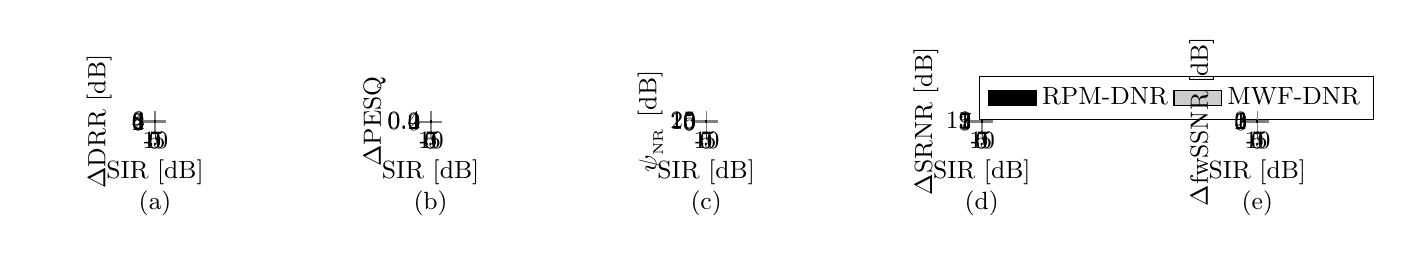
\begin{tikzpicture}[font = \small]

\begin{axis}[%
name = drr,
width=0.35\figurewidth,
height=0.8\figureheight,
scale only axis,
xmin=-8,
xmax=13,
xlabel absolute, xlabel style={align = center, text width=3cm, yshift=0.5em},
xlabel={SIR [dB] \\ (a)},
ylabel absolute, ylabel style={yshift=-1.5em},
xtick = {-5,0,5,10},
xticklabels = {-5,0,5,10},
ytick = {0, 2, 4, 6, 8, 10, 12},
yticklabels = {0, 2, 4, 6, 8, 10, 12},
xmajorgrids,
ymin=0,
ymax=8,
ylabel={$\Delta$DRR [dB]},
ymajorgrids
]

\addplot[ybar,bar width=0.0314285714285714\figurewidth,fill=black,draw=black] plot coordinates{(-6,7.52266732814821)
(-1,7.57908566903304)
(4,7.61437527860353)
(9,7.63639720827893)};

\addplot [
color=black,
solid,
forget plot
]
table[row sep=crcr]{
-8 0\\
8 0\\
};
\addplot[ybar,bar width=0.0314285714285714\figurewidth,fill=white!80!black,draw=black] plot coordinates{(-4,6.77367000052241)
(1,7.02344442478552)
(6,7.20292352547858)
(11,7.30184914397037)};

\end{axis}

\begin{axis}[%
name = pesq,
width=0.35\figurewidth,
height=0.8\figureheight,
scale only axis,
xmin=-8,
xmax=13,
xlabel absolute, xlabel style={align = center, text width=3cm, yshift=0.5em},
xlabel={SIR [dB] \\ (b)},
xtick = {-5,0, 5,10},
xticklabels = {-5,0,5,10},
ylabel absolute, ylabel style={yshift=-1.5em},
xmajorgrids,
ymin=0,
ymax=0.5,
ylabel={$\Delta$PESQ},
ymajorgrids,
at={($(drr.south east)+(3.5cm,0cm)$)},
anchor=south east,
]

\addplot[ybar,bar width=0.0314285714285714\figurewidth,fill=black,draw=black] plot coordinates{(-6,0.447333333333334)
(-1,0.4685)
(4,0.4755)
(9,0.470166666666667)};

\addplot [
color=black,
solid,
forget plot
]
table[row sep=crcr]{
-8 0\\
8 0\\
};
\addplot[ybar,bar width=0.0314285714285714\figurewidth,fill=white!80!black,draw=black] plot coordinates{(-4,0.413)
(1,0.431333333333333)
(6,0.443000000000001)
(11,0.448833333333333)};

\end{axis}

\begin{axis}[%
name = nr,
width=0.35\figurewidth,
height=0.8\figureheight,
scale only axis,
xmin=-8,
xmax=13,
xlabel absolute, xlabel style={align = center, text width=3cm, yshift=0.5em},
xlabel={SIR [dB] \\ (c)},
xtick = {-5,0,5,10},
xticklabels = {-5,0,5,10},
ylabel absolute, ylabel style={yshift=-1.5em},
xmajorgrids,
ymin=0,
ymax=19,
ylabel={$\psi_{_{\rm NR}}$ [dB]},
ymajorgrids,
at={($(pesq.south east)+(3.5cm,0cm)$)},
anchor=south east,
]

\addplot[ybar,bar width=0.0314285714285714\figurewidth,fill=black,draw=black] plot coordinates{(-6,7.61547770840405)
(-1,5.14831332899947)
(4,3.09628811037057)
(9,1.63887469885068)};

\addplot [
color=black,
solid,
forget plot
]
table[row sep=crcr]{
-8 0\\
8 0\\
};
\addplot[ybar,bar width=0.0314285714285714\figurewidth,fill=white!80!black,draw=black] plot coordinates{(-4,16.6581209881058)
(1,13.2248080958631)
(6,9.95223367941284)
(11,7.63259037560165)};


\end{axis}

\begin{axis}[%
name = sir,
width=0.35\figurewidth,
height=0.8\figureheight,
scale only axis,
xmin=-8,
xmax=13,
xtick = {-5,0,5,10},
xticklabels = {-5,0,5,10},
ytick = {3,5,7,9,11},
yticklabels = {3,5,7,9,11},
xlabel absolute, xlabel style={align = center, text width=3cm, yshift=0.5em},
xlabel={SIR [dB] \\ (d)},
ylabel absolute, ylabel style={yshift=-1.5em},
xmajorgrids,
ymin=1.5,
ymax=11,
%legend style={at={([yshift=0.5cm] $(nr.north west)!.5!(nr.north east)$)},anchor=north,row sep = -1pt,draw=black,fill=white,legend cell align=left, inner sep = 1pt},
legend style={at={(-2.0,1.1)},anchor=south west,legend cell align=left},
legend columns = 2,
area legend,
%legend image post style={xscale=0.8},
legend entries = {RPM-DNR, MWF-DNR},
at={($(nr.south east)+(3.5cm,0cm)$)},
anchor=south east,
ylabel={$\Delta$SRNR [dB]},
ymajorgrids
]
\addplot[ybar,bar width=0.0314285714285714\figurewidth,fill=black,draw=black] plot coordinates{(-6,5.65900439437402)
(-1,3.62944701930345)
(4,2.43643497060714)
(9,1.98425344336733)};

\addplot [
color=black,
solid,
forget plot
]
table[row sep=crcr]{
-8 0\\
8 0\\
};
\addplot[ybar,bar width=0.0314285714285714\figurewidth,fill=white!80!black,draw=black] plot coordinates{(-4,10.1905756183135)
(1,6.79895502348893)
(6,4.6166488576242)
(11,3.63616281528384)};

\end{axis}

\begin{axis}[%
name = fwssnr,
width=0.35\figurewidth,
height=0.8\figureheight,
scale only axis,
xmin=-8,
xmax=13,
xlabel absolute, xlabel style={align = center, text width=3cm, yshift=0.5em},
xlabel={SIR [dB] \\ (e)},
ylabel absolute, ylabel style={yshift=-1.5em},
xtick = {-5, 0, 5, 10},
xticklabels = {-5,0,5,10},
xmajorgrids,
ymin=0,
ymax=3,
ylabel={$\Delta$fwSSNR [dB]},
ymajorgrids,
at={($(sir.south east)+(3.5cm,0cm)$)},
anchor=south east,
]

\addplot[ybar,bar width=0.0314285714285714\figurewidth,fill=black,draw=black] plot coordinates{(-6,0.214826928764181)
(-1,0.758812887902899)
(4,1.19522269912336)
(9,1.37413374794192)};

\addplot [
color=black,
solid,
forget plot
]
table[row sep=crcr]{
-8 0\\
8 0\\
};
\addplot[ybar,bar width=0.0314285714285714\figurewidth,fill=white!80!black,draw=black] plot coordinates{(-4,2.77906764154485)
(1,2.81971178298215)
(6,2.64982879853452)
(11,2.29777409951572)};
\end{axis}

\end{tikzpicture}%
\caption{Average performance of the automatically parametrized RPM-DNR and MWF-DNR techniques in terms of (a) $\Delta$DRR, (b) $\Delta$PESQ of the output speech component, (c) $\psi_{_{\rm NR}} $, (d) $\Delta$SRNR, and (e) $\Delta$fwSSNR (simulated acoustic system, perfectly estimated correlation matrices).}
\label{fig: perfect}
\end{figure*}
\begin{figure*}[t!]
\centering
% This file was created by matlab2tikz v0.4.0.
% Copyright (c) 2008--2013, Nico Schlömer <nico.schloemer@gmail.com>
% All rights reserved.
% 
% The latest updates can be retrieved from
%   http://www.mathworks.com/matlabcentral/fileexchange/22022-matlab2tikz
% where you can also make suggestions and rate matlab2tikz.
% 
% 
%
\definecolor{mycolor1}{rgb}{1,0,1}%
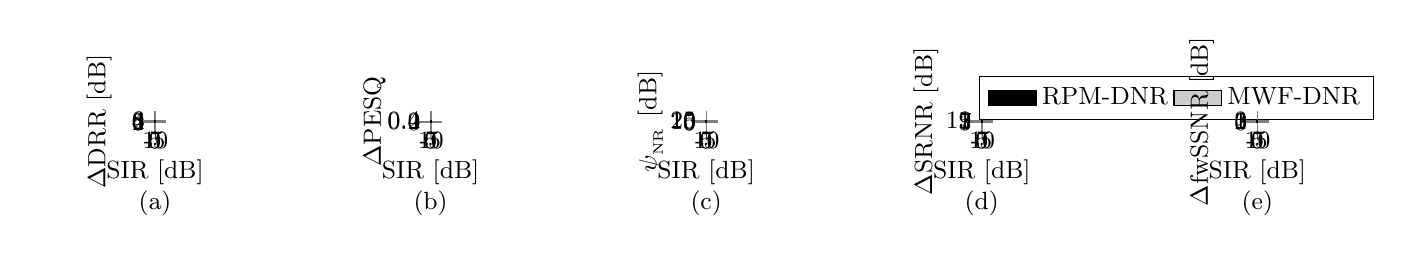
\begin{tikzpicture}[font = \small]

\begin{axis}[%
name = drr,
width=0.35\figurewidth,
height=0.8\figureheight,
scale only axis,
xmin=-8,
xmax=13,
xlabel absolute, xlabel style={align = center, text width=3cm, yshift=0.5em},
xlabel={SIR [dB] \\ (a)},
ylabel absolute, ylabel style={yshift=-1.5em},
xtick = {-5,0,5,10},
xticklabels = {-5,0,5,10},
ytick = {0, 2, 4, 6, 8, 10, 12},
yticklabels = {0, 2, 4, 6, 8, 10, 12},
xmajorgrids,
ymin=0,
ymax=8,
ylabel={$\Delta$DRR [dB]},
ymajorgrids
]

\addplot[ybar,bar width=0.0314285714285714\figurewidth,fill=black,draw=black] plot coordinates{(-6,7.5010851868773)
(-1,7.56463327596609)
(4,7.60592126447635)
(9,7.62864946524758)};

\addplot [
color=black,
solid,
forget plot
]
table[row sep=crcr]{
-8 0\\
8 0\\
};
\addplot[ybar,bar width=0.0314285714285714\figurewidth,fill=white!80!black,draw=black] plot coordinates{(-4,4.15487215260241)
(1,4.86398002211319)
(6,5.01667484164285)
(11,4.94431226602541)};

\end{axis}

\begin{axis}[%
name = pesq,
width=0.35\figurewidth,
height=0.8\figureheight,
scale only axis,
xmin=-8,
xmax=13,
xlabel absolute, xlabel style={align = center, text width=3cm, yshift=0.5em},
xlabel={SIR [dB] \\ (b)},
xtick = {-5,0, 5,10},
xticklabels = {-5,0,5,10},
ylabel absolute, ylabel style={yshift=-1.5em},
xmajorgrids,
ymin=0,
ymax=0.5,
ylabel={$\Delta$PESQ},
ymajorgrids,
at={($(drr.south east)+(3.5cm,0cm)$)},
anchor=south east,
]

\addplot[ybar,bar width=0.0314285714285714\figurewidth,fill=black,draw=black] plot coordinates{(-6,0.432666666666667)
(-1,0.4595)
(4,0.471833333333334)
(9,0.470833333333333)};

\addplot [
color=black,
solid,
forget plot
]
table[row sep=crcr]{
-8 0\\
8 0\\
};
\addplot[ybar,bar width=0.0314285714285714\figurewidth,fill=white!80!black,draw=black] plot coordinates{(-4,0.0611666666666668)
(1,0.191333333333334)
(6,0.267666666666667)
(11,0.315166666666667)};

\end{axis}

\begin{axis}[%
name = nr,
width=0.35\figurewidth,
height=0.8\figureheight,
scale only axis,
xmin=-8,
xmax=13,
xlabel absolute, xlabel style={align = center, text width=3cm, yshift=0.5em},
xlabel={SIR [dB] \\ (c)},
xtick = {-5,0,5,10},
xticklabels = {-5,0,5,10},
ylabel absolute, ylabel style={yshift=-1.5em},
xmajorgrids,
ymin=0,
ymax=19,
ylabel={$\psi_{_{\rm NR}}$ [dB]},
ymajorgrids,
at={($(pesq.south east)+(3.5cm,0cm)$)},
anchor=south east,
]

\addplot[ybar,bar width=0.0314285714285714\figurewidth,fill=black,draw=black] plot coordinates{(-6,7.71926146995955)
(-1,5.26170396863151)
(4,3.25741759950274)
(9,1.82934452864539)};

\addplot [
color=black,
solid,
forget plot
]
table[row sep=crcr]{
-8 0\\
8 0\\
};
\addplot[ybar,bar width=0.0314285714285714\figurewidth,fill=white!80!black,draw=black] plot coordinates{(-4,13.4688613303205)
(1,12.4942812240601)
(6,10.7682679204459)
(11,8.93880725901647)};


\end{axis}

\begin{axis}[%
name = sir,
width=0.35\figurewidth,
height=0.8\figureheight,
scale only axis,
xmin=-8,
xmax=13,
xtick = {-5,0,5,10},
xticklabels = {-5,0,5,10},
ytick = {3,5,7,9,11},
yticklabels = {3,5,7,9,11},
xlabel absolute, xlabel style={align = center, text width=3cm, yshift=0.5em},
xlabel={SIR [dB] \\ (d)},
ylabel absolute, ylabel style={yshift=-1.5em},
xmajorgrids,
ymin=1.5,
ymax=11,
%legend style={at={([yshift=0.5cm] $(nr.north west)!.5!(nr.north east)$)},anchor=north,row sep = -1pt,draw=black,fill=white,legend cell align=left, inner sep = 1pt},
legend style={at={(-2.0,1.1)},anchor=south west,legend cell align=left},
legend columns = 2,
area legend,
%legend image post style={xscale=0.8},
legend entries = {RPM-DNR, MWF-DNR},
at={($(nr.south east)+(3.5cm,0cm)$)},
anchor=south east,
ylabel={$\Delta$SRNR [dB]},
ymajorgrids
]
\addplot[ybar,bar width=0.0314285714285714\figurewidth,fill=black,draw=black] plot coordinates{(-6,5.66937009120099)
(-1,3.65113811240757)
(4,2.48265737725432)
(9,2.02933931964001)};


\addplot [
color=black,
solid,
forget plot
]
table[row sep=crcr]{
-8 0\\
8 0\\
};
\addplot[ybar,bar width=0.0314285714285714\figurewidth,fill=white!80!black,draw=black] plot coordinates{(-4,7.32261595607633)
(1,5.70030303309397)
(6,4.23069307824245)
(11,3.48015398938991)};

\end{axis}

\begin{axis}[%
name = fwssnr,
width=0.35\figurewidth,
height=0.8\figureheight,
scale only axis,
xmin=-8,
xmax=13,
xlabel absolute, xlabel style={align = center, text width=3cm, yshift=0.5em},
xlabel={SIR [dB] \\ (e)},
ylabel absolute, ylabel style={yshift=-1.5em},
xtick = {-5, 0, 5, 10},
xticklabels = {-5,0,5,10},
xmajorgrids,
ymin=0,
ymax=3,
ylabel={$\Delta$fwSSNR [dB]},
ymajorgrids,
at={($(sir.south east)+(3.5cm,0cm)$)},
anchor=south east,
]

\addplot[ybar,bar width=0.0314285714285714\figurewidth,fill=black,draw=black] plot coordinates{(-6,0.144055722658052)
(-1,0.730074705953759)
(4,1.19348885980111)
(9,1.38086149822489)};


\addplot [
color=black,
solid,
forget plot
]
table[row sep=crcr]{
-8 0\\
8 0\\
};
\addplot[ybar,bar width=0.0314285714285714\figurewidth,fill=white!80!black,draw=black] plot coordinates{(-4,1.46720411543849)
(1,2.24446496367937)
(6,2.69372250380039)
(11,2.62610745645293)};

\end{axis}

\end{tikzpicture}%
\caption{Average performance of the automatically parametrized RPM-DNR and MWF-DNR techniques in terms of (a) $\Delta$DRR, (b) $\Delta$PESQ of the output speech component, (c) $\psi_{_{\rm NR}} $, (d) $\Delta$SRNR, and (e) $\Delta$fwSSNR (simulated acoustic system, erroneously estimated correlation matrices).}
\label{fig: estimate}
\end{figure*}
To illustrate the importance of taking the RIR perturbations and the noise statistics into account, in this section the performance of the automatically parametrized RPM-DNR and MWF-DNR techniques is compared to the performance of the PMINT and the automatically regularized PMINT techniques using the simulated acoustic system for an exemplary scenario of SIR $= 0$~dB and NPM = $-33$~dB. 
The speech and noise correlation matrices for the RPM-DNR and MWF-DNR techniques are perfectly estimated as in~(\ref{eq: corr}).

Table~\ref{tbl: perf} presents the obtained $\Delta$DRR, $\Delta$PESQ, $\psi_{_{\rm NR}}$, $\Delta$SRNR, and $\Delta$fwSSNR values for all considered techniques.
As shown by the negative $\Delta$DRR and $\Delta$PESQ values, PMINT fails to achieve dereverberation, introducing more reverberant energy than in the microphone signal.
By taking the RIR perturbations into account, RPMINT achieves a high reverberant energy suppression and perceptual speech quality improvement.
The proposed RPM-DNR technique achieves a very similar dereverberation performance as RPMINT, whereas the proposed MWF-DNR technique yields only a slightly worse dereverberation performance. 
Even though one would expect the dereverberation performance of the RPM-DNR technique to be worse than the dereverberation performance of RPMINT, in this scenario the dereverberation performance of both techniques is very similar. 
This occurs due to the automatic selection of the regularization parameter, which does not yield the best dereverberation performance one would otherwise obtain by intrusively selecting the regularization parameter in the RPMINT technique.
Furthermore, as discussed in Section~\ref{sec: eq} and as illustrated by the negative noise reduction factor, PMINT leads to a large noise amplification.
Due to the decrease in the reshaping filter energy by incorporating a regularization parameter, RPMINT avoids the noise amplification and reduces the noise by $1.9$~dB.
By taking the noise statistics explicitly into account, the proposed RPM-DNR technique improves the noise reduction factor to $3.2$~dB, whereas by taking also the reverberant speech statistics into account the proposed MWF-DNR technique yields a significantly larger noise reduction factor of $13.0$~dB. 
The high dereverberation and noise reduction performance of the proposed techniques in comparison to acoustic multi-channel equalization techniques is also illustrated by the higher $\Delta$SRNR and $\Delta$fwSSNR values presented in Table~\ref{tbl: perf}, where the MWF-DNR technique outperforms the RPM-DNR technique in terms of both instrumental measures. 
Summarizing these results, it can be said that the RIR perturbations and the noise statistics should be taken into account in order to avoid noise amplification and to achieve joint dereverberation and noise reduction.
By taking also the reverberant speech statistics into account, an overall better performance can be achieved.

\subsection{Performance of the automatically parametrized RPM-DNR and MWF-DNR techniques for simulated acoustic systems}
\label{sec: expc}
In this section the performance of the automatically parametrized RPM-DNR and MWF-DNR techniques is extensively investigated using the simulated acoustic system for different noise levels, RIR perturbation levels, and correlation matrix estimation errors. 
The considered NPMs are given in~(\ref{eq: npm}) and the presented performance measures for each SIR value are averaged over the different considered NPMs. 
The performance of the proposed RPM-DNR and MWF-DNR techniques is investigated for perfectly estimated correlation matrices as in~(\ref{eq: corr}) and for erroneously estimated correlation matrices as in~(\ref{eq: corrdiff}).

Fig.~\ref{fig: perfect} depicts the performance of the automatically parametrized RPM-DNR and MWF-DNR techniques for perfectly estimated speech and noise correlation matrices.
As shown by the $\Delta$DRR and $\Delta$PESQ values in Figs.~\ref{fig: perfect}a and~\ref{fig: perfect}b, the dereverberation performance of both techniques is very similar, with the RPM-DNR technique yielding a slightly better performance.
However, as shown by the noise reduction factor in Fig.~\ref{fig: perfect}c, the MWF-DNR technique achieves a significantly better noise reduction performance.
\begin{table*}[t]
  \def\tabcolsep{8pt}
  \caption{Performance of the automatically parametrized RPM-DNR and MWF-DNR techniques~(recorded acoustic system, erroneously estimated correlation matrices).}
  \label{tbl: ssi}
  \begin{tabularx}{\linewidth}{rrrrrrrrrr}
    \toprule
& &    \multicolumn{2}{c}{$\Delta$DRR [dB]} & \multicolumn{2}{c}{$\Delta$PESQ} & \multicolumn{2}{c}{$\eta_{_{\text{NR}}}$ [dB]} & \multicolumn{2}{c}{$\Delta$fwSSNR [dB]} \\
    \midrule
  SIR [dB] & NPM [dB] & RPM-DNR & MWF-DNR &  RPM-DNR & MWF-DNR & RPM-DNR & MWF-DNR & RPM-DNR & MWF-DNR \\
    $-5$ & $-3.0$ & $\bf{6.0}$ & $3.9$ & $\bf{0.2}$ & $-0.1$ & $5.9$ & $\bf{16.4}$ & $0.6$ & $\bf{3.8}$ \\
    $0$ & $-4.5$ & $\bf{6.8}$ & $5.2$ & $\bf{0.5}$ & $0.0$ & $4.4$ & $\bf{12.7}$ & $1.1$ & $\bf{4.7}$ \\
    $5$ & $-5.2$ & $\bf{7.4}$ & $6.0$ & $\bf 0.7$ & $0.2$ & $3.3$ & $\bf{9.9}$ & $1.6$ & $\bf{5.7}$ \\
    $10$ & $-5.5$ & $\bf{7.8}$ & $6.8$ & $\bf 0.8$ & $0.4$ & $2.4$ & $\bf{8.0}$ & $1.7$ & $\bf{6.6}$ \\
    $10$ & $-\infty$ & $\bf{8.4}$ & $6.8$ & $\bf 0.8$ & $0.3$  & $1.5$ & $\bf{8.0}$ & $1.0$ & $\bf{5.6}$ \\
    \bottomrule
  \end{tabularx}
\end{table*}
The similar dereverberation performance but better noise reduction performance of the MWF-DNR technique is reflected in the higher $\Delta$SRNR and $\Delta$fwSSNR values achieved by the MWF-DNR technique, as depicted in Figs.~\ref{fig: perfect}d and~\ref{fig: perfect}e.
Hence, it can be said that by also taking the true reverberant speech statistics into account, the MWF-DNR technique outperforms the RPM-DNR technique, since it yields a similarly high dereverberation performance but a significantly higher noise reduction performance. 


Fig.~\ref{fig: estimate} depicts the performance of the automatically parametrized RPM-DNR and MWF-DNR techniques for erroneously estimated correlation matrices as in~(\ref{eq: corrdiff}).
{{Since the RPM-DNR technique only requires the noise correlation matrix $\mathbf{R}_{\mathbf{v}}$ and since estimating this matrix from a long enough spatially stationary noise-only period does not yield a significantly different estimate from the previous experiment, the performance of the RPM-DNR technique for erroneously estimated correlation matrices is very similar to the performance for perfectly estimated correlation matrices (compare Figs.~\ref{fig: perfect} and~\ref{fig: estimate}).}}
However, as shown in Figs.~\ref{fig: estimate}a and~\ref{fig: estimate}b the dereverberation performance of the MWF-DNR technique significantly decreases.
Due to the fact that the speech and noise signals are not perfectly uncorrelated and the noise is temporally nonstationary, estimation errors occur in the estimate of the speech correlation matrix $\mathbf{R}_{\mathbf{x}} = \mathbf{R}_{\mathbf{y}} - \mathbf{R}_{\mathbf{v}}$, especially for low input SIR.
These estimation errors result in a worse dereverberated reference signal $\mathbf{R}_{\mathbf{x}}\mathbf{w}_{_{\rm RP}}$ for the MWF-DNR technique, hence, significantly decreasing the dereverberation performance. 
However, the noise reduction performance for the MWF-DNR technique is significantly better than for the RPM-DNR technique as depicted in Fig.~\ref{fig: estimate}c, resulting in higher overall $\Delta$SRNR and $\Delta$fwSSNR values as depicted in Figs.~\ref{fig: estimate}d and~\ref{fig: estimate}e.
Furthermore, the noise reduction performance of the MWF-DNR technique for erroneously estimated correlation matrices can be better than for perfectly estimated correlation matrices~(compare Figs.~\ref{fig: perfect}c and~\ref{fig: estimate}c for SIR = $5$ dB and SIR = $10$ dB).
This occurs due to the automatic selection of the weighting parameter $\mu$ in the MWF-DNR technique, which for erroneously estimated correlation matrices may result in a higher parameter value, hence a better noise reduction performance (at the expense of a worse dereverberation performance).

{{In summary, when the speech and noise correlation matrices can be directly estimated from the speech and noise signals, the MWF-DNR technique outperforms the RPM-DNR technique since it yields a similarly high dereverberation performance and a significantly better noise reduction performance. 
However, when the required correlation matrices are prone to estimation errors, the RPM-DNR technique yields a significantly better dereverberation performance but still a worse noise reduction performance than the MWF-DNR technique.}} 
The technique to be used should be chosen depending on what is more important for the application under consideration, i.e., dereverberation or noise reduction performance. 

{{
\subsection{Performance of the automatically parametrized RPM-DNR and MWF-DNR techniques for recorded acoustic systems}
\label{sec: expd}
In this section the performance of the automatically parametrized RPM-DNR and MWF-DNR techniques is investigated using the recorded acoustic system for different noise levels, and hence, different RIR perturbations, cf.~(\ref{eq: err_ssi}).
The correlation matrices are erroneously estimated as in~(\ref{eq: corrdiff}).

Table~\ref{tbl: ssi} presents the obtained $\Delta$DRR, $\Delta$PESQ, $\eta_{_{\text{NR}}}$, and $\Delta$fwSSNR values for both proposed techniques.
It should be noted that the presented $\Delta$PESQ values do not only reflect the improvement in dereverberation performance, but also the reduction of ambient noise and microphone self-noise (since for the recorded acoustic system, the individual speech, ambient noise or microphone self-noise components are not available).
For each considered SIR, the NPM arising between the measured RIRs and the estimated RIRs is also presented in Table~\ref{tbl: ssi}.
As a baseline, the performance of the RPM-DNR and MWF-DNR techniques using the measured RIRs (i.e., NPM $=-\infty$) for the exemplary scenario of SIR = $10$ dB is also presented.

As illustrated by the $\Delta$DRR and $\Delta$PESQ values and as expected from the results of Section~\ref{sec: expc}, the RPM-DNR technique yields a better dereverberation performance than the MWF-DNR technique.
Furthermore, as illustrated by the $\eta_{_{\text{NR}}}$ values, the MWF-DNR technique yields a better noise reduction performance than the RPM-DNR technique.
The better noise reduction performance of the MWF-DNR technique also results in a better overall joint dereverberation and noise reduction performance, as illustrated by the $\Delta$fwSSNR values.
Most importantly, it can be observed that at SIR = $10$ dB the performance of both techniques for NPM = $-5.5$ dB is very similar to the performance for NPM = $-\infty$ dB, illustrating the robustness of the proposed techniques against RIR perturbations arising due to least-squares SSI.

In summary, these simulation results confirm the results of Section~\ref{sec: expc}, i.e., in the presence of correlation matrix estimation errors, the RPM-DNR technique yields a significantly better dereverberation performance whereas the MWF-DNR technique yields a significantly better noise reduction and joint dereverberation and noise reduction performance.
Most importantly, these simulation results show the applicability of the proposed techniques to more realistic acoustic scenarios, with realistic RIR perturbations arising from SSI methods.
}}
\section{Conclusion}
In this paper we have proposed two techniques for joint dereverberation and noise reduction based on acoustic multi-channel equalization.
The RPM-DNR technique can be seen as an extension of the RPMINT technique by explicitly taking the noise statistics into account. 
The MWF-DNR technique takes also the reverberant speech statistics into account and uses the dereverberated output signal of the RPMINT technique as the reference signal for the MWF.
In addition, we proposed an automatic non-intrusive procedure based on the L-hypersurface for selecting the regularization and weighting parameters in the RPM-DNR technique, whereas two decoupled procedures based on the L-curve were used for the automatic selection of the parameters in the MWF-DNR technique.
Simulation results demonstrate that the RPM-DNR technique maintains the high dereverberation performance of acoustic multi-channel equalization techniques while improving the noise reduction performance. 
Furthermore, it is shown that the MWF-DNR technique yields a significantly better noise reduction performance than the RPM-DNR technique at the expense of a worse dereverberation performance, depending on the amount of estimation errors in the speech correlation matrix.

\bibliographystyle{IEEEtran}
\bibliography{refs}

\begin{IEEEbiography}[{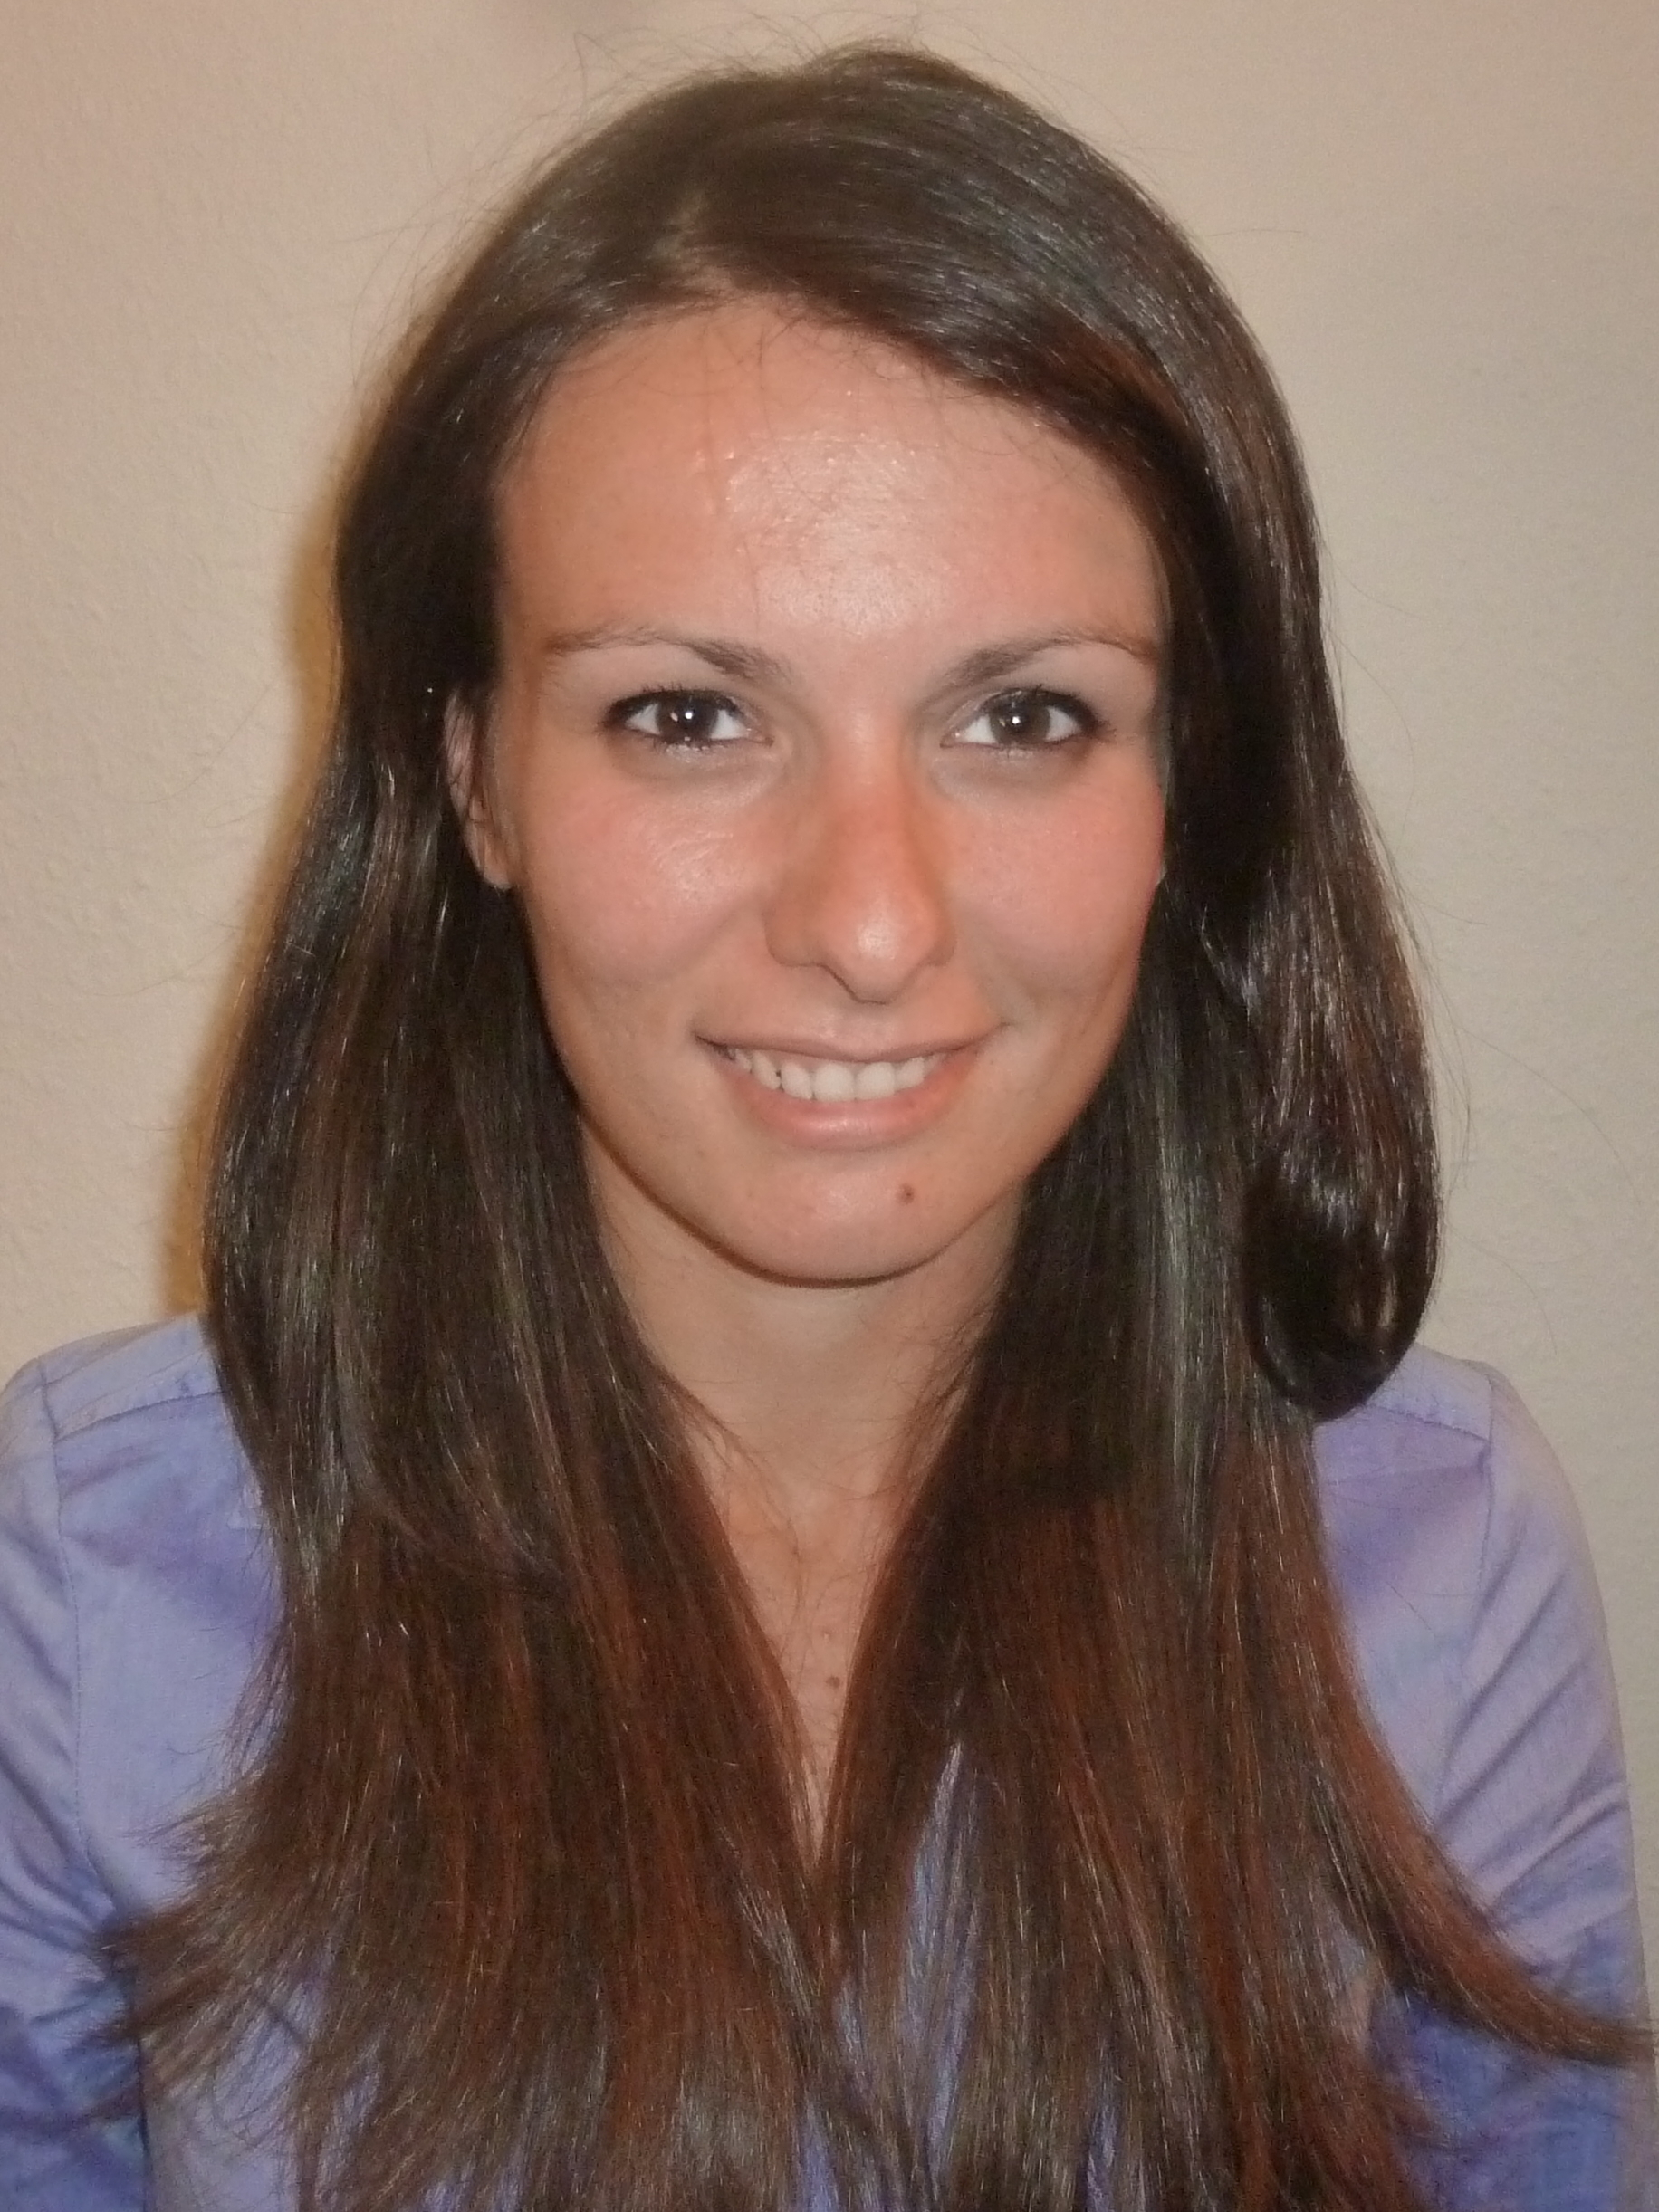
\includegraphics[width=1in,height=1.25in,clip,keepaspectratio]{Plots2/ina1}}]
{Ina Kodrasi} received the Master of Science degree in Communications, Systems and Electronics in 2010 from Jacobs University Bremen, Germany.
Currently she is a PhD student at the Signal Processing Group of the University of Oldenburg, Germany.
Her research interests are in the area of signal processing for speech and audio applications.
From 2010 to 2011 she was also with the Fraunhofer Institute for Digital Media Technology (IDMT), Project group
Hearing, Speech and Audio Technology in Oldenburg where she worked on microphone-array beamforming.
\end{IEEEbiography}

\begin{IEEEbiography}[{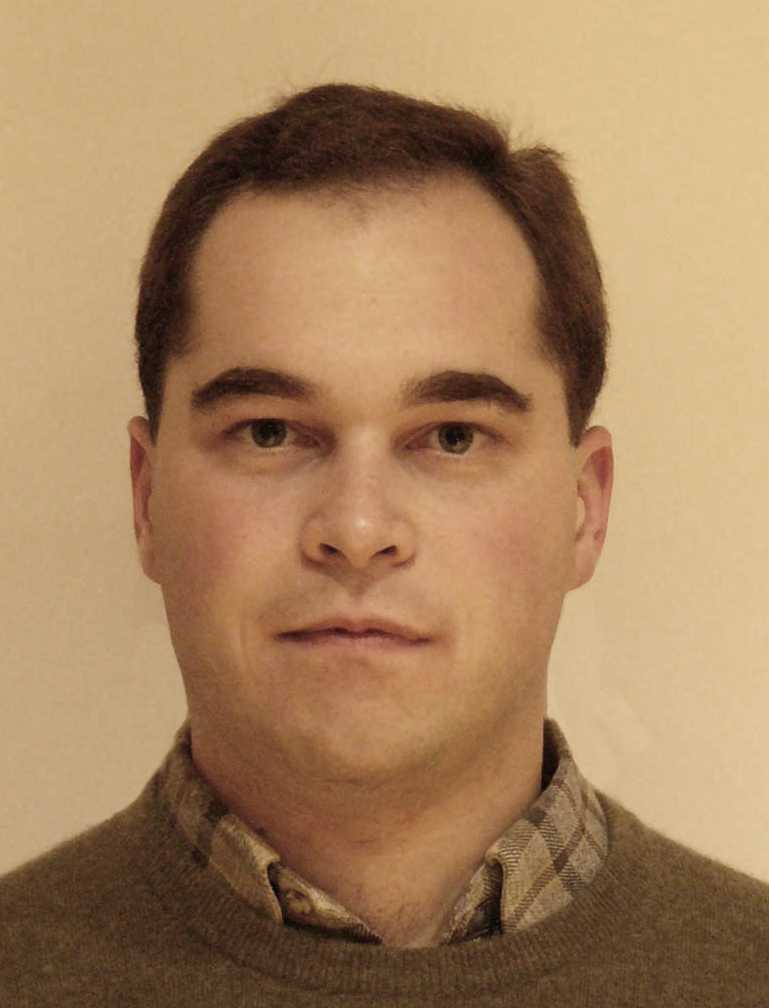
\includegraphics[width=1in,height=1.25in,clip,keepaspectratio]{Plots2/sd}}]{Simon Doclo}
(S'95, M'03) received the M.Sc. degree in electrical engineering and the Ph.D. degree in applied sciences from the Katholieke Universiteit Leuven, Belgium, in 1997 and 2003. From 2003 to 2007 he was a Postdoctoral Fellow with the Research Foundation-Flanders at the Electrical Engineering Department (Katholieke Universiteit Leuven) and the Adaptive Systems Laboratory (McMaster University, Canada). From 2007 to 2009 he was a Principal Scientist with NXP Semiconductors at the Sound and Acoustics Group in Leuven, Belgium. Since 2009 he is a full professor at the University of Oldenburg, Germany, and scientific advisor for the project group Hearing, Speech and Audio Technology of the Fraunhofer Institute for Digital Media Technology. His research activities center around signal processing for acoustical applications, more specifically microphone array processing, active noise control, acoustic sensor networks and hearing aid processing.
Prof. Doclo received the Master Thesis Award of the Royal Flemish Society of Engineers in 1997 (with Erik De Clippel), the Best Student Paper Award at the International Workshop on Acoustic Echo and Noise Control in 2001, the EURASIP Signal Processing Best Paper Award in 2003 (with Marc Moonen) and the IEEE Signal Processing Society 2008 Best Paper Award (with Jingdong Chen, Jacob Benesty, Arden Huang). He is a member of the IEEE Signal Processing Society Technical Committee on Audio and Acoustic Signal Processing (2008-2013). He has been secretary of the IEEE Benelux Signal Processing Chapter (1998-2002), and has served as a guest editor for the EURASIP Journal on Applied Signal Processing.
\end{IEEEbiography}

\end{document}


